\chapter{Results}
\label{ch:results}
This chapter presents the statistical analysis where the results
for each case-study, such as mascot-speakers, mascot-lamp, mascot-mascot, and
mascot-tablet are reported in separate sections.
Each section consists of two subsections describing tests for two
studies: the within personality traits study and the within conditions such as types of music, lighting colors,
vibration levels, or screen colors.

Since the gathered data are ordinal and the outcome
is not normally distributed, the analysis of all case-studies is focused on the non-parametric tests.
Specifically, since each case-study consists of more than two compared groups
(i.e.\ each described in Sections~\ref{sec:m-s}, ~\ref{sec:m-l}, ~\ref{sec:m-m}, and ~\ref{sec:m-t})
and data is compared against a within-subject factor (i.e.\ each participant tested all conditions),
the Friedman tests followed by the Wilcoxon Signed-rank tests are used for statistical analysis.

For each study, the Wilcoxon tests compare 10 groups with each other except from a
study one for the mascot-speakers interaction where it compares 6 groups.
Since there are a large number of statistical tests,
some of the results may have p<.05 purely by chance.
Thus, in order to control the family-wise error rate, the Bonferroni
correction is used.
This adjustment method will divide all p-values in 10 and 6 according to the number of compared groups.

In addition, in each subsection, the results of Wilcoxon tests after Bonferroni correction are
displayed graphically using box plots.
The complete tables of these tests can be found in appendices (see Appendix~\ref{ch:tables-and-figures}).

% p\textsubscript{adj}
%%%%%%%%%%%%%%%%%%%%%%%%%%%%%%%%%%%%%%%%%%%%%%%%%%%%%%%%%%%%%%%%%%%%%%%%%%%%%%%%%%%%%%%%%%%%%%%%%%%%%%%%%%%%%%%%%%%%%%%%
\section{The analysis of the mascot-speakers interaction.}
\label{sec:m-s}
This section describes the mascot-speakers case-study, where is analyzed the effect of music
on the measurement of the mascots' personality traits.
As discussed in Section~\ref{sec:Identifying the music preferences based on the personality traits},
the choice of the music genre is based on the MUSIC pattern.
For statistical analysis, all songs that were used in the experiments are
distributed into the following categories:
\begin{itemize}
    \item Sophisticated: jazz, classical and contemporary adult.
    \item Contemporary: rap and soul.
    \item Unpretentious: pop, rock\&roll / country and bluegrass.
\end{itemize}

In addition, the raw data consists of 30 personality facets for each music condition
(see Section~\ref{sec:Identifying personality traits}).
During analysis, all facets are grouped into five personality traits.
Thus, each personality trait consists of the mean scores given for six personality facets.
The analysis of the mascot-speakers interaction is performed by two studies.

In the first study, we compare three types of music within each personality trait
to find the effects of each music on participant's measurements of mascot's personality.
In the second study, the second iteration on the same dataset is performed by comparing five personality traits
within each music category.

Figure~\ref{fig:Stat12} depicts both studies for mascot-speakers interaction where vertical arrows represent the first study
i.e.\ analysis of the within personality trait and horizontal arrows represent the analysis of the within condition study.
In the first study, we determine the effect of music on the measurements of personality traits.
Thus, we compare all music types with each other within a specific personality trait.
It results in music that is significantly different and rated higher in comparison to all other music types.
Since we compare all conditions within each personality separately (see vertical arrows in Figure~\ref{fig:Stat12}),
one music may be associated with multiple personality traits.
We aim to conclude with one music condition being associated with a specific personality trait.
In the second study, we compare all personality traits within each music type (see horizontal
arrows in Figure~\ref{fig:Stat12}) which helps us to find personality trait that is conveyed by specific music most.

In addition, we apply the same statistical tests for each case-study
(see Sections ~\ref{sec:m-l}, ~\ref{sec:m-m}, and ~\ref{sec:m-t}).

\begin{figure}[hbt!]
    \centering
    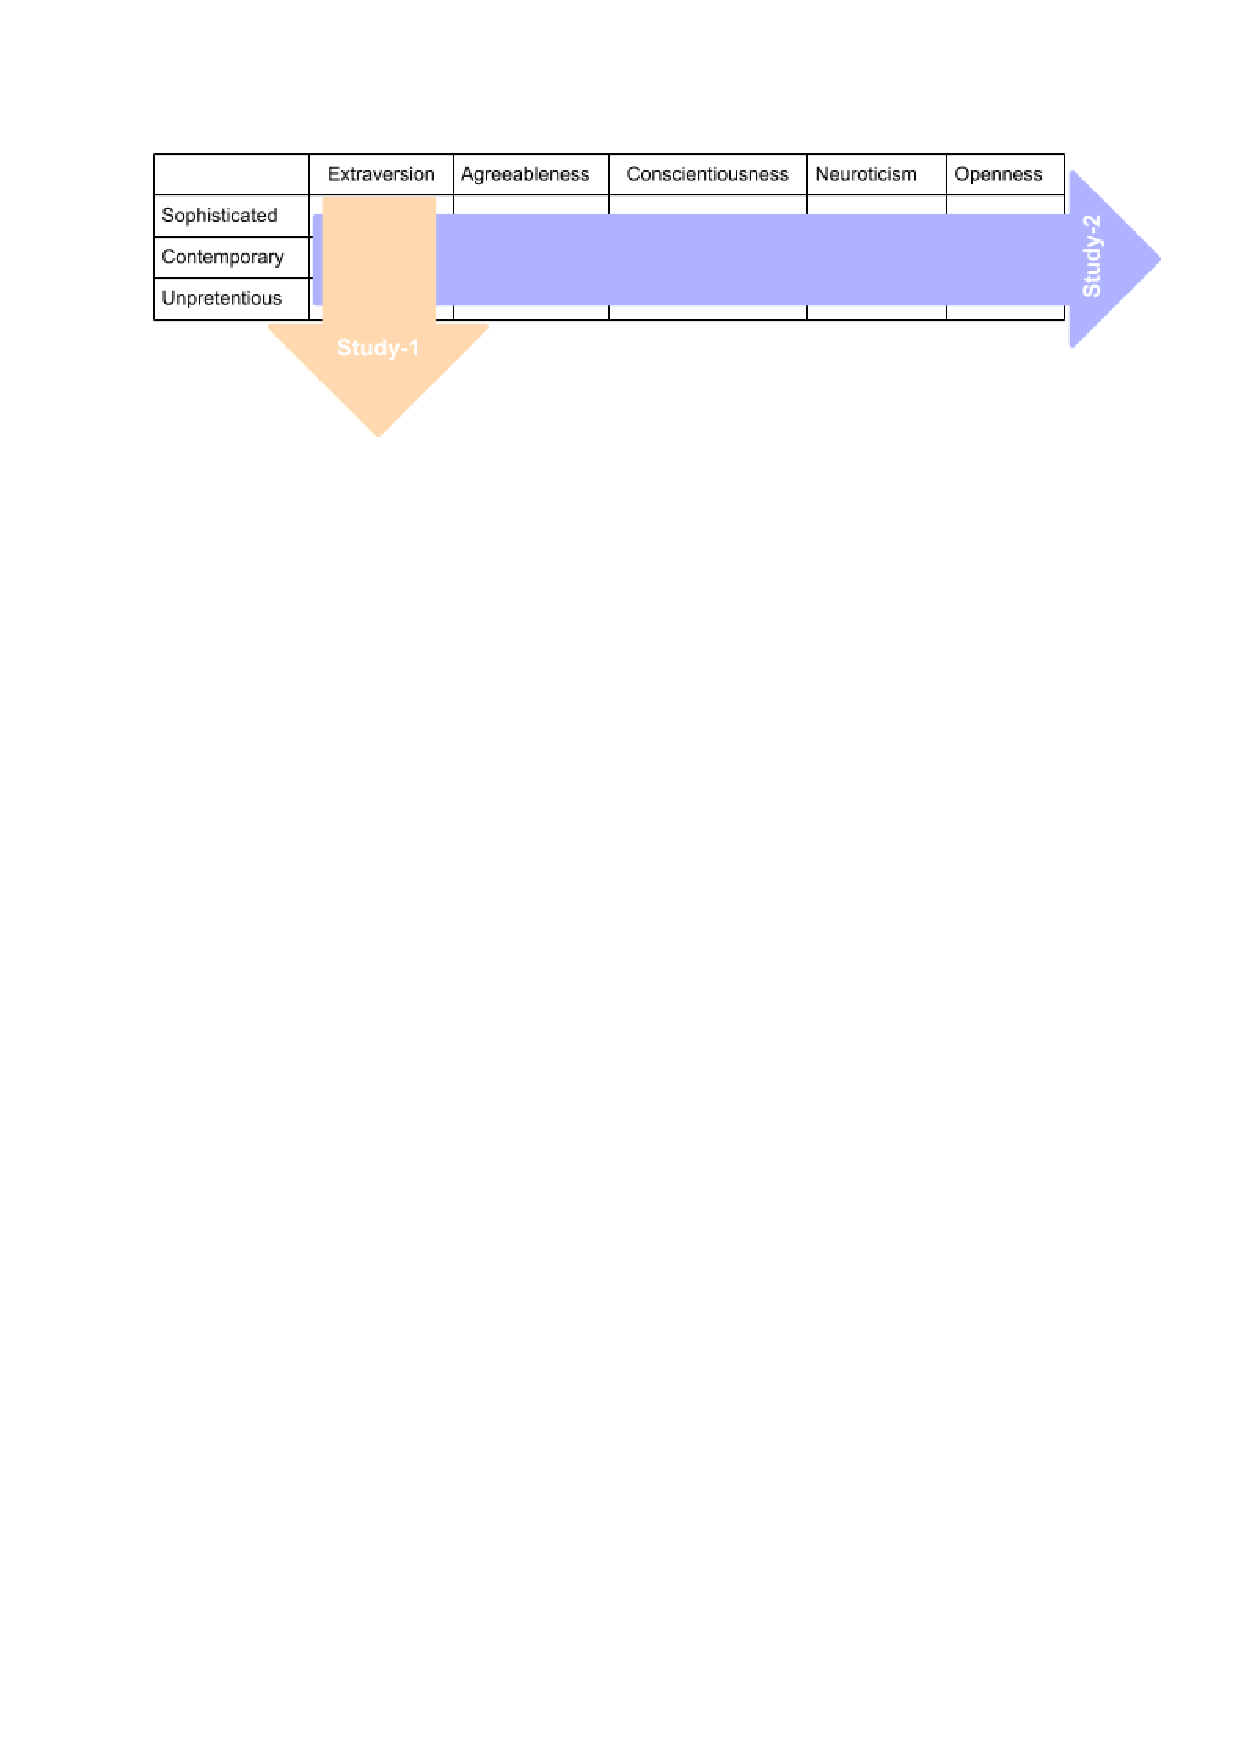
\includegraphics[scale=0.65]{StatSt12.pdf}
    \caption{Visual representation of compared groups in study-1 for vertical arrows and
    study-2 for horizontal arrows in case of mascot-speakers interaction.}
    \label{fig:Stat12}
\end{figure}

In this chapter, the abbreviations for all tables
(i.e.\ Tables ~\ref{table:medianMS1} - ~\ref{table:medianMT2},) and figures
(i.e.\ Figures ~\ref{fig:MS1} - ~\ref{fig:MT2}) are described in the footnotes
\footnote[1]{The abbreviations for stars: $^{**}$ p\textsubscript{adj}<.01 and $^{*}$ p\textsubscript{adj}<.05}
\footnote[2]{The abbreviations for personality traits: $^{E}$ extraversion, $^{A}$ agreeableness, $^{C}$ conscientiousness, $^{N}$ neuroticism
and $^{O}$ openness personality trait}
\footnote[3]{The abbreviations for music types: $^{S}$ sophisticated, $^{C}$ contemporary, $^{U}$ unpretentious music}
\footnote[4]{The abbreviations for vibrations: $^{L1}$ vibration level-1, $^{L2}$ level-2, $^{L3}$ level-3, $^{L4}$ level-4 and $^{L5}$ level-5}
\footnote[5]{The abbreviations for colors: $^{Y}$ yellow, $^{O}$ orange, $^{T}$ turquoise, $^{B}$ blood-red and $^{P}$ pink color}.
%%%%%%%%%%%%%%%%%%%%%%%%%%%%%%%%%%%%%%%%%%%%%%%%%%%%%%%%%%%%%%%%%%%
\subsection{The analysis of the within personality trait study.}
\label{subsec:MSstudy1}
In this subsection, we report a statistical analysis of how the impact of the music category varies within each
personality trait.
Compared factors are sophisticated, contemporary, and unpretentious music.

\par\textbf{Extraversion.}
The Friedman tests show the significant effect of all predefined music categories on the
ratings of extraversion personality with p<.01, df=2 (see Table~\ref{table:friedmanMS1}).
The Wilcoxon tests revealed that the significant difference is concentrated on contemporary music
compared to all other categories with p\textsubscript{adj}<.01 (see Figure~\ref{fig:MS1}).
According to Table~\ref{table:medianMS1}, the contemporary category has the highest median with med = 3.9.

\par\textbf{Agreeableness.}
All three categories significantly influenced participants' measurements of mascot's
agreeableness personality trait with p<.01, df=2 (see Table~\ref{table:friedmanMS1}).
The main difference fault in the following groups: sophisticated and contemporary;
contemporary and unpretentious with p<.01.
According to Figure~\ref{fig:MS1}, the boxplot distinguishes most of the contemporary samples from
the other two categories having very low ratings to convey the agreeableness personality trait.

\par\textbf{Conscientiousness.}
There is a significant difference in all music categories within conscientiousness
personality trait with p<.05, df=2 (see Table~\ref{table:friedmanMS1}.
Scores for mascot being measured as conscientiousness personality trait increased sharply during playing
sophisticated and unpretentious (med = 3.2) music in comparison to scores for contemporary music (med = 2.8)
The Wilcoxon test confirms the statistically significant difference between the following groups:
sophisticated and contemporary (p\textsubscript{adj}<.01); unpretentious and contemporary (p\textsubscript{adj}<.05).

\par\textbf{Neuroticism.}
Overall, all three categories have an effect on the measurement of mascot's neuroticism
personality with p<.01, df=2 (see Table~\ref{table:friedmanMS1}).
Table~\ref{table:medianMS1} shows that the scores given for contemporary music while assessing
neuroticism personality traits are the highest with med = 3.1 compared to the other two categories.
Moreover, there are two significant differences between groups: sophisticated and contemporary;
contemporary and unpretentious music with p\textsubscript{adj}<.01 (see Figure~\ref{fig:MS1}).

\par\textbf{Openness.}
Table~\ref{table:friedmanMS1} reveals a substantial difference between all three music types
within an openness personality trait.
Particularly, there is a good separation of the sophisticated with med = 3.8 and max = 4.9
from other music categories (see Table~\ref{table:medianMS1}).
There is a large difference between sophisticated and contemporary, and sophisticated
and unpretentious with p\textsubscript{adj}<.01 (see Figure~\ref{fig:MS1}).

\begin{table}[hbt!]
    \renewcommand{\arraystretch}{1}
    \begin{center}
        \begin{tabular}{|c|c|c|c|}
            \hline
            \textbf{Personality traits} & \textbf{$\chi^2$} & \textbf{df} & \textbf{p} \\
            \hline
            Extraversion &21.4 &2 &p<.01 \\
            \hline
            Agreeableness &29.0 &2 &p<.01\\
            \hline
            Conscientiousness &6.5 &2 &p<.05\\
            \hline
            Neuroticism &15.1 &2 &p<.01 \\
            \hline
            Openness &25.8 &2 &p<.01 \\
            \hline
        \end{tabular}
        \caption{The results of the Friedman test for five personality traits in the case of mascot-speakers interaction.}
        \label{table:friedmanMS1}
    \end{center}
\end{table}

\begin{table}[hbt!]
    \renewcommand{\arraystretch}{1}
    \begin{center}
        \begin{tabular}{p{0.05\textwidth}|
        p{0.025\textwidth}|p{0.025\textwidth}|p{0.025\textwidth}||
        p{0.025\textwidth}|p{0.025\textwidth}|p{0.025\textwidth}||
        p{0.025\textwidth}|p{0.025\textwidth}|p{0.025\textwidth}||
        p{0.025\textwidth}|p{0.025\textwidth}|p{0.025\textwidth}||
        p{0.025\textwidth}|p{0.025\textwidth}|p{0.025\textwidth}|}
            \cline{2-16}
            & \multicolumn{3}{c||}{\textbf{E}} & \multicolumn{3}{c||}{\textbf{A}}
            & \multicolumn{3}{c||}{\textbf{C}} &  \multicolumn{3}{c||}{\textbf{N}} & \multicolumn{3}{c|}{\textbf{O}} \\
            \cline{2-16}
            & S & C & U & S & C & U & S & C & U & S & C & U & S & C & U            \\
            \cline{2-16}
            \textbf{Min}    & 1.4 & 3.2 & 2.2 & 2.9 & 1.1 & 2.5 & 2.4 & 1.0 & 1.9 & 1.0 & 2.3 & 1.3 & 3.1 & 2.0 & 2.5 \\
            \textbf{Med}    & 3.1 & 3.9 & 3.3 & 3.3 & 2.9 & 3.7 & 3.2 & 2.8 & 3.2 & 2.4 & 3.1 & 2.5 & 3.8 & 2.9 & 3.4\\
            \textbf{Max}    & 3.8 & 5.0 & 4.0 & 4.7 & 4.3 & 4.7 & 4.6 & 4.0 & 4.7 & 3.4 & 4.5 & 3.2 & 4.9 & 4.0 & 4.7\\
            \cline{2-16}
        \end{tabular}
        \caption{A summary table of the median, minimum, and maximum rates given for each personality trait.}
        \label{table:medianMS1}
    \end{center}
\end{table}
%%%%%%
%%%%%%
\begin{figure}[hbt!]
    \centering
    \begin{subfigure}{.45\textwidth}
        \centering
        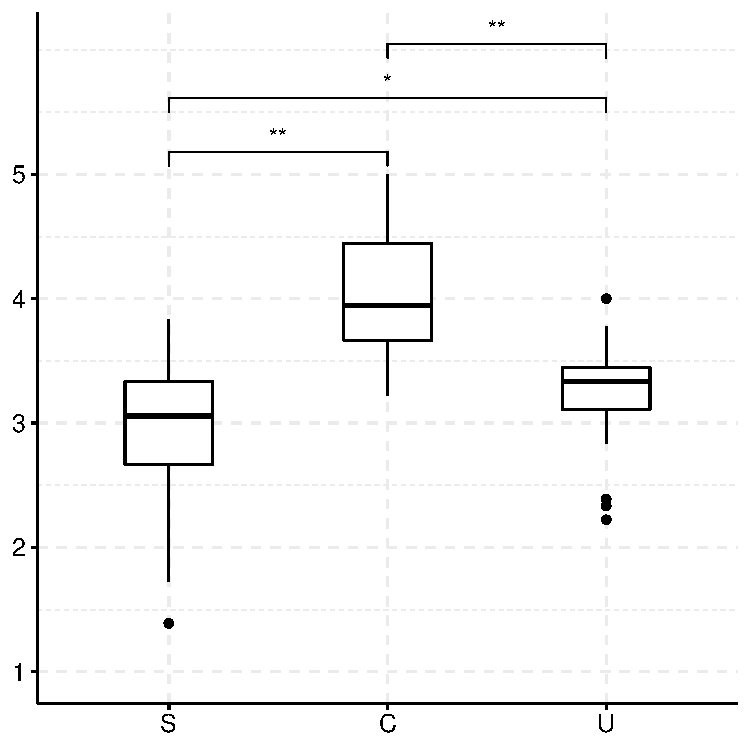
\includegraphics[width=1\linewidth]{M_S_Study_1_Extrav.pdf}
        \caption{Extraversion}
        \label{fig:sub1}
    \end{subfigure}\hfill%
    \begin{subfigure}{.45\textwidth}
        \centering
        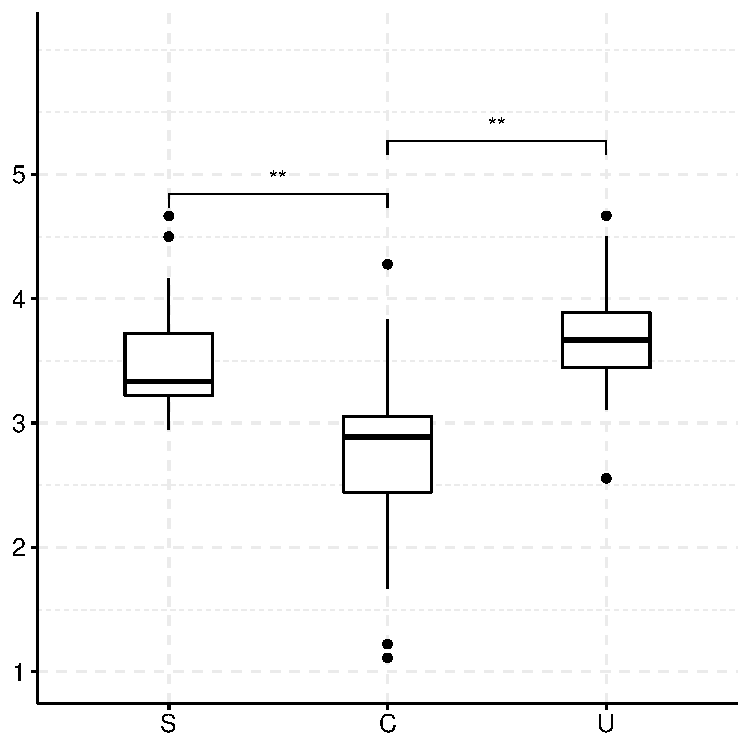
\includegraphics[width=1\linewidth]{M_S_Study_1_Agreeab.pdf}
        \caption{Agreeableness}
        \label{fig:sub2}
    \end{subfigure}\hfill
    \begin{subfigure}{.45\textwidth}
        \centering
        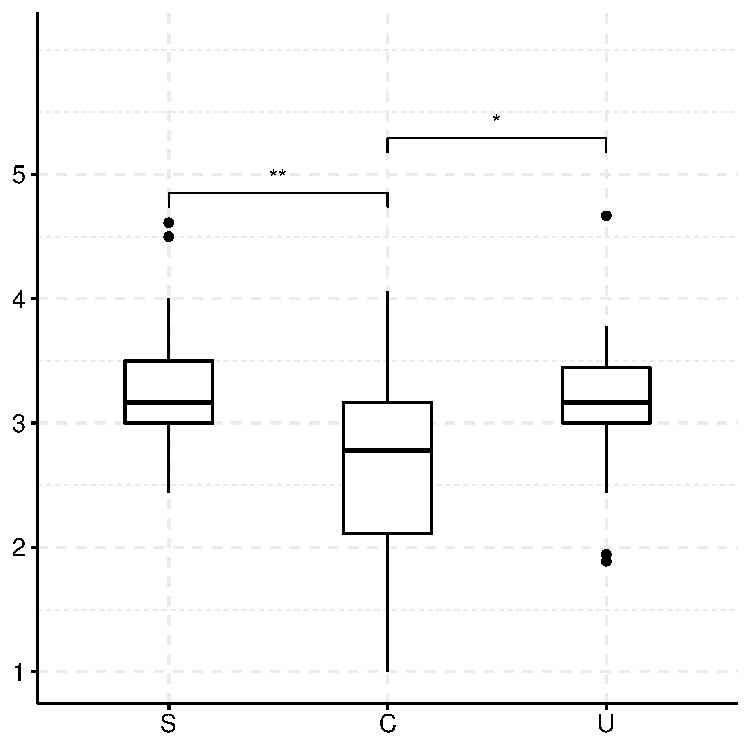
\includegraphics[width=1\linewidth]{M_S_Study_1_Consc.pdf}
        \caption{Conscientiousness}
        \label{fig:sub1}
    \end{subfigure}\hfill%
    \begin{subfigure}{.45\textwidth}
        \centering
        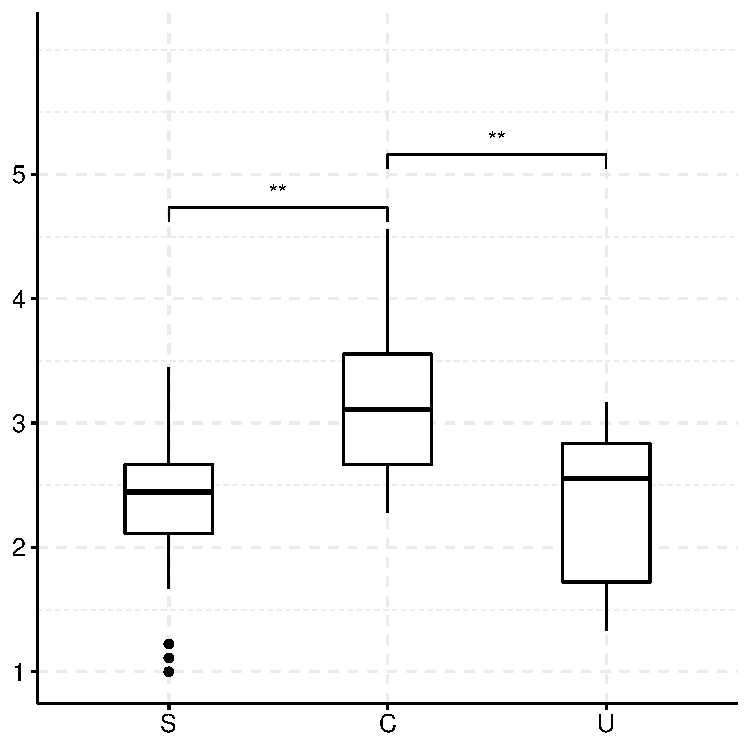
\includegraphics[width=1\linewidth]{M_S_Study_1_Neurot.pdf}
        \caption{Neuroticism}
        \label{fig:sub1}
    \end{subfigure}\hfill%
    \begin{subfigure}{.45\textwidth}
        \centering
        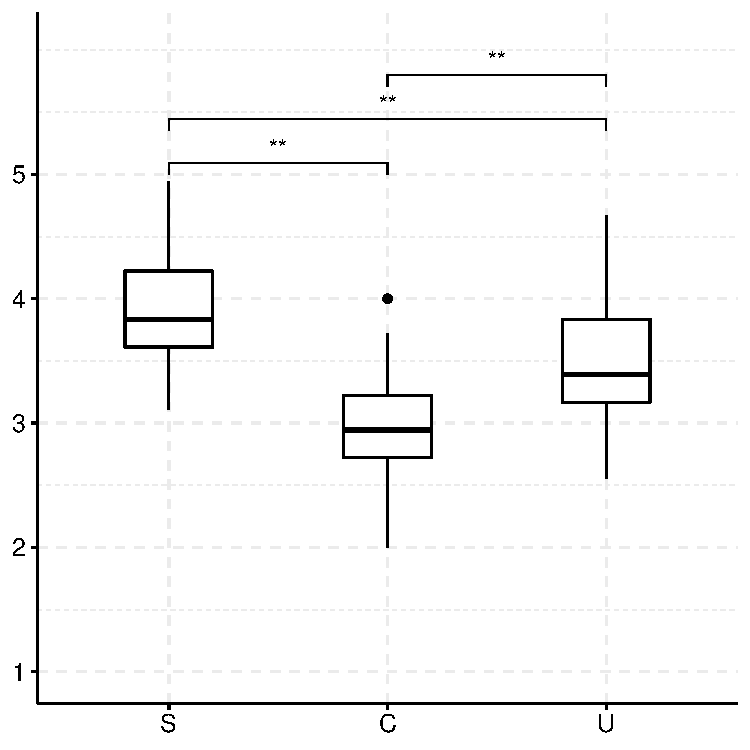
\includegraphics[width=1\linewidth]{M_S_Study_1_Open.pdf}
        \caption{Openness}
        \label{fig:sub1}
    \end{subfigure}\hfill%
    \caption{A boxplot for the mascot-speakers interaction in study-1.
    Stars represent the significance of p\textsubscript{adj} after Bonferroni correction.}
    \label{fig:MS1}
\end{figure}
%%%%%%%%%%%%%%%%%%%%%%%%%%%%%%%%%%%%%%%%%%%%%%%%%%%%%%%%%%%%%%%%%%%
\subsection{The analysis of the within music category study.}
\label{subsec:MSstudy2}
In this study, we analyze the effect of each music category, particularly on how each personality
trait is assessed differently within one music condition.
Compared groups are extraversion, agreeableness, conscientiousness, neuroticism, and openness personality traits.

\par\textbf{Sophisticated.}
On average, sophisticated music has a significant effect on all five personality traits with
p<.01, df=2 (see Table~\ref{table:friedmanMS2}).
When sophisticated is played, in comparison to all the personality traits,
openness is rated very high with med = 3.8, and neuroticism
is rated very low with med = 2.4 (see Table~\ref{table:medianMS2}).
According to Figure~\ref{fig:MS2}, openness to experience shows a
significant difference from all other personality traits in the group.

\par\textbf{Contemporary.}
The Friedman test shows a significant difference between the ratings of all personality traits and
contemporary music with p<.01, df=2 (see Table~\ref{table:friedmanMS2}).
According to Figure~\ref{fig:MS2}, for mascot triggering contemporary music, there is a clear
separation of extraversion samples from all other personality traits with p\textsubscript{adj}<.01.
The median value for extraversion is very high being med = 3.9 compared to all
other personality traits (med $\approx$ 3).

\par\textbf{Unpretentious}
music substantially affects the measurements of all personality traits with
p<.01, df=4 (see Table~\ref{table:friedmanMS2}).
Based on Wilcoxon tests, neuroticism personality trait is rated very low when unpretentious music
was played with p\textsubscript{adj}<.01 (see Figure~\ref{fig:MS2}).
The median values of all other personality traits slightly differ from each other,
condensed around 'neutral' rating which is med $\approx$ 3 (see Table~\ref{table:medianMS2}).

\begin{table}[hbt!]
    \renewcommand{\arraystretch}{1}
    \begin{center}
        \begin{tabular}{|c|c|c|c|}
            \hline
            \textbf{Music categories} & \textbf{$\chi^2$} & \textbf{df} & \textbf{p} \\
            \hline
            Sophisticated &66.6 &4 &p<.01 \\
            \hline
            Contemporary &44.4 &4 &p<.01\\
            \hline
            Unpretentious &57.4 &4 &p<.01 \\
            \hline
        \end{tabular}
        \caption{The results of the Friedman test for all music categories in the case of mascot-speakers interaction.}
        \label{table:friedmanMS2}
    \end{center}
\end{table}

\begin{table}[hbt!]
    \renewcommand{\arraystretch}{1}
    \begin{center}
        \begin{tabular}{p{0.05\textwidth}|
        p{0.025\textwidth}|p{0.025\textwidth}|p{0.025\textwidth}|p{0.025\textwidth}|p{0.025\textwidth}||
        p{0.025\textwidth}|p{0.025\textwidth}|p{0.025\textwidth}|p{0.025\textwidth}|p{0.025\textwidth}||
        p{0.025\textwidth}|p{0.025\textwidth}|p{0.025\textwidth}|p{0.025\textwidth}|p{0.025\textwidth}|}
            \cline{2-16}
            & \multicolumn{5}{c||}{\textbf{Sophisticated}} & \multicolumn{5}{c||}{\textbf{Contemporary}}
            & \multicolumn{5}{c|}{\textbf{Unpretentious}} \\
            \cline{2-16}
            & E & A & C & N & O & E & A & C & N & O & E & A & C & N & O     \\
            \cline{2-16}
            \textbf{Min}    & 1.4 & 2.9 & 2.4 & 1.0 & 3.1 & 3.2 & 1.1 & 1.0 & 2.3 & 2.0 & 2.2 & 2.5 & 1.9 & 1.3 & 2.5  \\
            \textbf{Med}    & 3.0 & 3.3 & 3.2 & 2.4 & 3.8 & 3.9 & 2.9 & 2.8 & 3.1 & 2.9 & 3.3 & 3.7 & 3.2 & 2.5 & 3.4   \\
            \textbf{Max}    & 3.8 & 4.7 & 4.6 & 3.4 & 4.9 & 5.0 & 4.3 & 4.0 & 4.5 & 4.0 & 4.0 & 4.7 & 4.7 & 3.2 & 4.7 \\
            \cline{2-16}
        \end{tabular}
        \caption{A summary table of the median, minimum, and maximum rates given for each music category.}
        \label{table:medianMS2}
    \end{center}
\end{table}
%%%%%%
\begin{figure}[hbt!]
    \centering
    \begin{subfigure}{.45\textwidth}
        \centering
        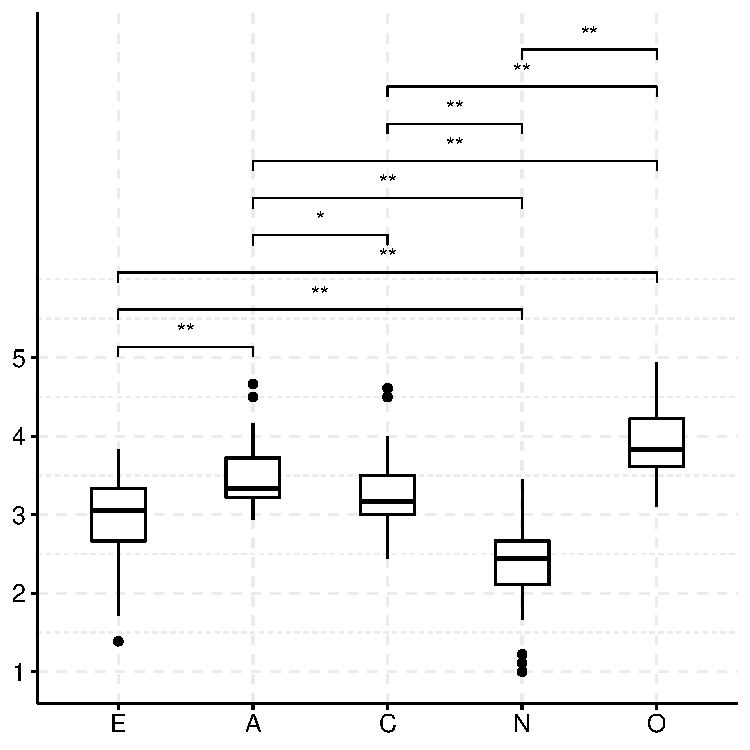
\includegraphics[width=1\linewidth]{M_S_Study_2_Sop.pdf}
        \caption{Sophisticated}
        \label{fig:sub1}
    \end{subfigure}\hfill%
    \begin{subfigure}{.45\textwidth}
        \centering
        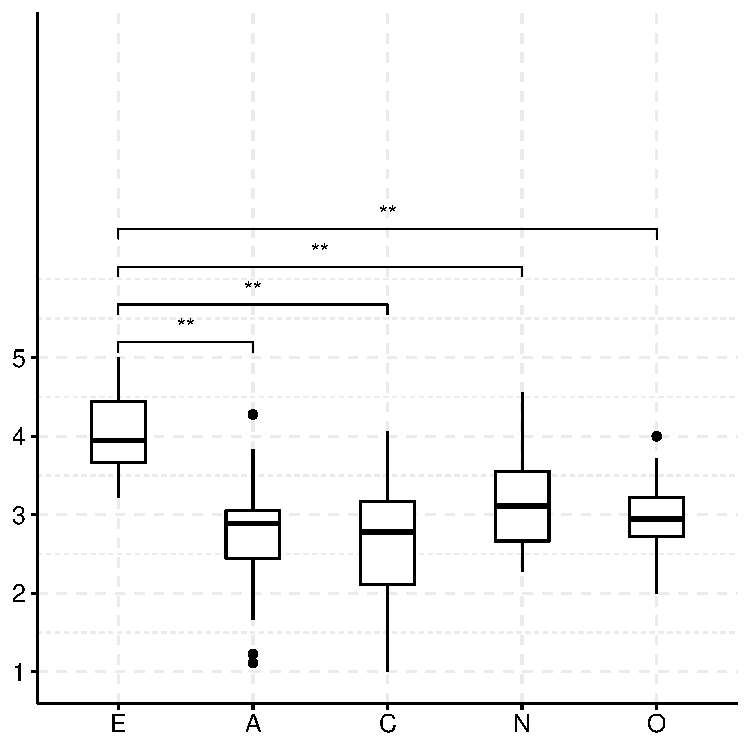
\includegraphics[width=1\linewidth]{M_S_Study_2_Con.pdf}
        \caption{Contemporary}
        \label{fig:sub2}
    \end{subfigure}\hfill
    \begin{subfigure}{.45\textwidth}
        \centering
        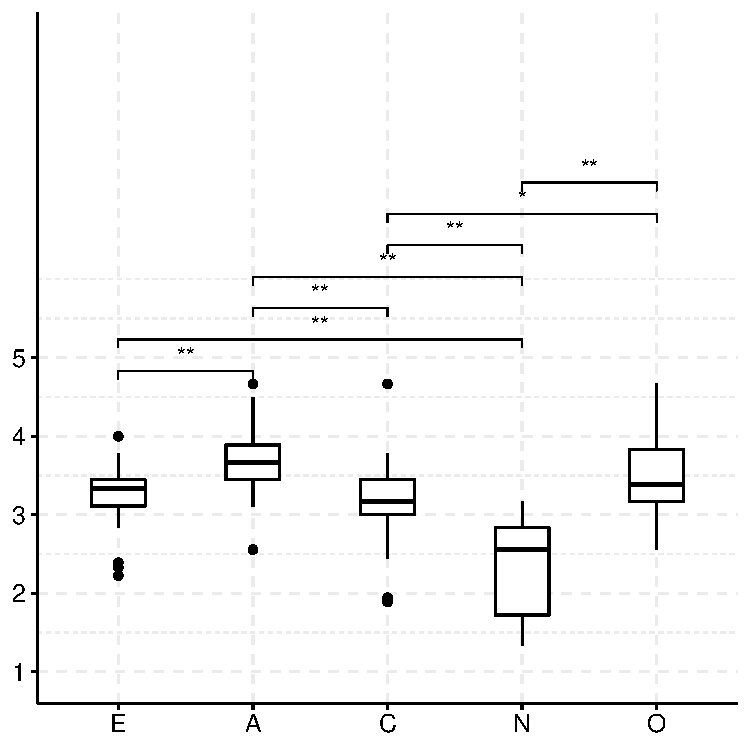
\includegraphics[width=1\linewidth]{M_S_Study_2_Unp.pdf}
        \caption{Unpretentious}
        \label{fig:sub1}
    \end{subfigure}\hfill%
    \caption{A boxplot for the mascot-speakers interaction in study-2.
    Stars represent the significance of p\textsubscript{adj} after Bonferroni correction.}
    \label{fig:MS2}
\end{figure}
%%%%%%%%%%%%%%%%%%%%%%%%%%%%%%%%%%%%%%%%%%%%%%%%%%%%%%%%%%%%%%%%%%%%%%%%%%%%%%%%%%%%%%%%%%%%%%%%%%%%%%%%%%%%%%%%%%%%%%%%
\section{The analysis of the mascot-lamp interaction.}
\label{sec:m-l}
This section investigates the effect of the lighting color on the measurement of the mascots' personality traits.
Subsection~\ref{subsec:MLstudy1} describes the results for the within personality study and
subsection~\ref{subsec:MLstudy2} for the within the lighting color study.

%%%%%%%%%%%%%%%%%%%%%%%%%%%%%%%%%%%%%%%%%%%%%%%%%%%%%%%%%%%%%%%%%%%
\subsection{The analysis of the within personality trait study.}
\label{subsec:MLstudy1}
In the first study, that compared factors are orange, turquoise, yellow, blood-red, and pink lighting colors.

\par\textbf{Extraversion.}
According to Table~\ref{table:friedmanML1}, all lighting colors significantly
influenced the measurements of extraversion personality with p<.01, df=4.
Figure~\ref{fig:ML1} shows where exactly this effect is concentrated
reporting six groups of colors with p\textsubscript{adj}<.01.
Yellow showed a significant difference compared to turquoise, blood-red and pink lighting colors
being rated very high on conveying extraversion personality trait.
In contrast, the mascot interacting with blood-red lighting was rated very low on being an extravert.
This is also reported in Table~\ref{table:medianML1}, the blood-red color having
the lowest median (med = 1.7, max = 4.5, min = 1.0) and yellow having the highest
value (med = 3.7, max = 4.8, min = 2.3) for extraversion personality.

\par\textbf{Agreeableness.}
There is a significant impact of lighting colors and the participants'
measurements of agreeableness personality with p<.01 (see Table~\ref{table:friedmanML1})
According to Figure~\ref{fig:ML1}, in comparison to all other colors,
mascots triggering blood-red and orange lighting
are rated very low to have an agreeableness personality (p\textsubscript{adj}<.01).
Moreover, Table~\ref{table:medianML1} shows that compared to all other colors,
blood-red has the smallest median with med = 2.0.
The median values, in descending order, for pink, turquoise, and yellow lights are
approximately similar with med = 4.0, med = 3.5 and med = 3.7 respectively.

\par\textbf{Conscientiousness.}
The Friedman test shows a statistically significant effect of all predefined lighting colors
on the ratings of conscientiousness personality (see Table~\ref{table:friedmanML1}).
The Wilcoxon tests show that effect is noticeable when we compare mascot that triggers
blood-red and orange with ones that triggered turquoise, yellow, pink colors (see Figure~\ref{fig:ML1}).
In fact, the mascot interacting blood-red and orange were assessed
as being very low on the conscientious personality trait.
Table~\ref{table:medianML1} indicates that blood-red has the lowest median (med = 2.2), whereas turquoise, pink and
yellow have relatively similar high medians (med = 3.7, med = 3.5, med = 3.5 respectively).
The latest values show that the mascot triggering these colors is rated high on having
orderly, dutiful, disciplined, and other facets that constitute conscientiousness personality.

\par\textbf{Neuroticism.}
Overall, there is an impact of the predefined colors on the ratings of the neuroticism
personality with p<.01 reported in Table~\ref{table:friedmanML1}.
The blood-red color showed a significant difference in rating neuroticism comparing
to all other colors with p\textsubscript{adj}<.01 (see Figure~\ref{fig:ML1}).
Moreover, blood-red presents the highest values with med = 4.3, max = 5.0, min = 3.2 (see Table~\ref{table:medianML1}).

\par\textbf{Openness.}
There is a significant difference of all colors within openness personality
with p<.01 (see Table~\ref{table:friedmanML1}).
The main differences are concentrated between the following groups: yellow and pink;
yellow and blood-red;
blood-red and orange with p\textsubscript{adj}<.01 (see Figure~\ref{fig:ML1}).
Table~\ref{table:medianML1} shows the similarity of the median values for all colors concentrating around neutral attitude for mascot
being measured as openness which is represented by med $\approx$ 3.

\begin{table}[hbt!]
    \renewcommand{\arraystretch}{1}
    \begin{center}
        \begin{tabular}{|c|c|c|c|}
            \hline
            \textbf{Personality traits} & \textbf{$\chi^2$} & \textbf{df} & \textbf{p} \\
            \hline
            Extraversion &40.0 &4 & p<.01 \\
            \hline
            Agreeableness &56.4 &4 & p<.01 \\
            \hline
            Conscientiousness &25.8 &4 & p<.01\\
            \hline
            Neuroticism &52.4 &4 & p<.01 \\
            \hline
            Openness &18.2 &4 & p<.01 \\
            \hline
        \end{tabular}
        \caption{The results of the Friedman test for all personality traits for the first study
        in the case of mascot-lamp interaction.}
        \label{table:friedmanML1}
    \end{center}
\end{table}

\begin{table}[hbt!]
    \renewcommand{\arraystretch}{1}
    \begin{center}
        \begin{tabular}{p{0.05\textwidth}|
        p{0.025\textwidth}|p{0.025\textwidth}|p{0.025\textwidth}|p{0.025\textwidth}|p{0.025\textwidth}||
        p{0.025\textwidth}|p{0.025\textwidth}|p{0.025\textwidth}|p{0.025\textwidth}|p{0.025\textwidth}||
        p{0.025\textwidth}|p{0.025\textwidth}|p{0.025\textwidth}|p{0.025\textwidth}|p{0.025\textwidth}|}
            \cline{2-16}
            & \multicolumn{5}{c||}{\textbf{Extraversion}} & \multicolumn{5}{c||}{\textbf{Agreeableness}}
            & \multicolumn{5}{c|}{\textbf{Conscientiousness}} \\
            \cline{2-16}
            & Y & O & T & B & P & Y & O & T & B & P & Y & O & T & B & P     \\
            \cline{2-16}
            \textbf{Min}    & 2.3 & 2.3 & 1.8 & 1.0 & 1.7 & 1.8 & 1.0 & 2.0 & 1.0 & 2.5 & 1.3 & 1.8 & 1.7 & 1.2 & 2.0  \\
            \textbf{Med}    & 3.7 & 3.0 & 2.7 & 1.7 & 2.8 & 3.7 & 2.3 & 3.5 & 2.0 & 4.0 & 3.5 & 2.5 & 3.7 & 2.2 & 3.5  \\
            \textbf{Max}    & 4.8 & 4.8 & 4.2 & 4.5 & 3.7 & 5.0 & 3.3 & 5.0 & 3.8 & 5.0 & 4.8 & 3.3 & 5.0 & 4.7 & 5.0 \\
            \cline{2-16}
            \cline{2-11}
            &  \multicolumn{5}{|c||}{\textbf{Neuroticism}} & \multicolumn{5}{|c||}{\textbf{Openness}} \\
            \cline{2-11}
            & Y & O & T & B & P & Y & O & T & B & P            \\
            \cline{2-11}
            \textbf{Min}    & 1.0 & 1.0 & 1.0 & 3.2 & 1.0 & 1.5 & 1.7 & 2.3 & 1.2 & 1.5    \\
            \textbf{Med}    & 2.1 & 2.5 & 2.0 & 4.3 & 1.7 & 3.5 & 3.0 & 2.8 & 2.7 & 2.8    \\
            \textbf{Max}    & 3.3 & 3.5 & 3.5 & 5.0 & 3.3 & 5.0 & 4.7 & 3.7 & 4.0 & 4.0    \\
            \cline{2-11}
        \end{tabular}
        \caption{A summary table of the median, minimum, and maximum rates given for each personality trait.}
        \label{table:medianML1}
    \end{center}
\end{table}
%%%
\begin{figure}[hbt!]
    \centering
    \begin{subfigure}{.45\textwidth}
        \centering
        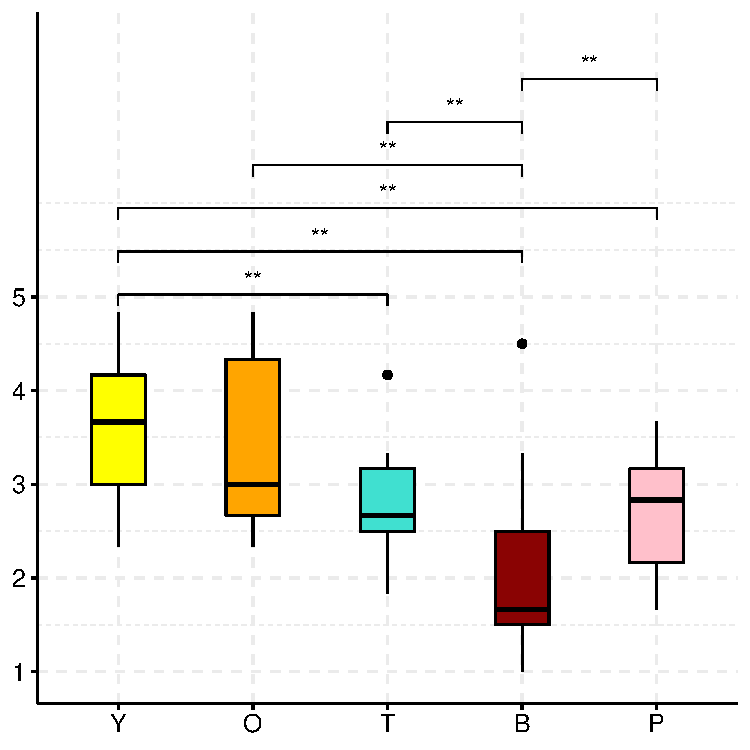
\includegraphics[width=1\linewidth]{M_L_Study_1_Extrav.pdf}
        \caption{Extraversion}
        \label{fig:sub1}
    \end{subfigure}\hfill%
    \begin{subfigure}{.45\textwidth}
        \centering
        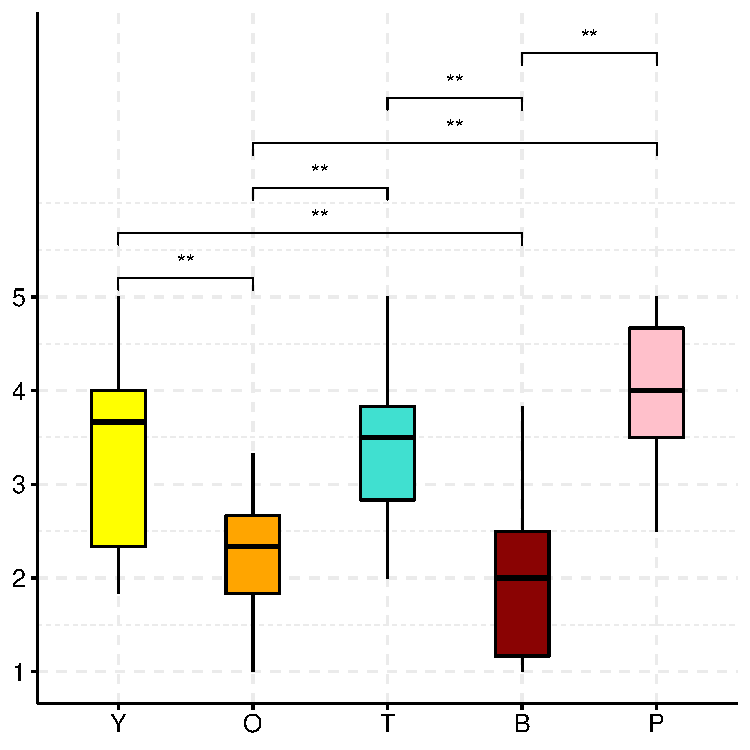
\includegraphics[width=1\linewidth]{M_L_Study_1_Agreeab.pdf}
        \caption{Agreeableness}
        \label{fig:sub2}
    \end{subfigure}\hfill
    \begin{subfigure}{.45\textwidth}
        \centering
        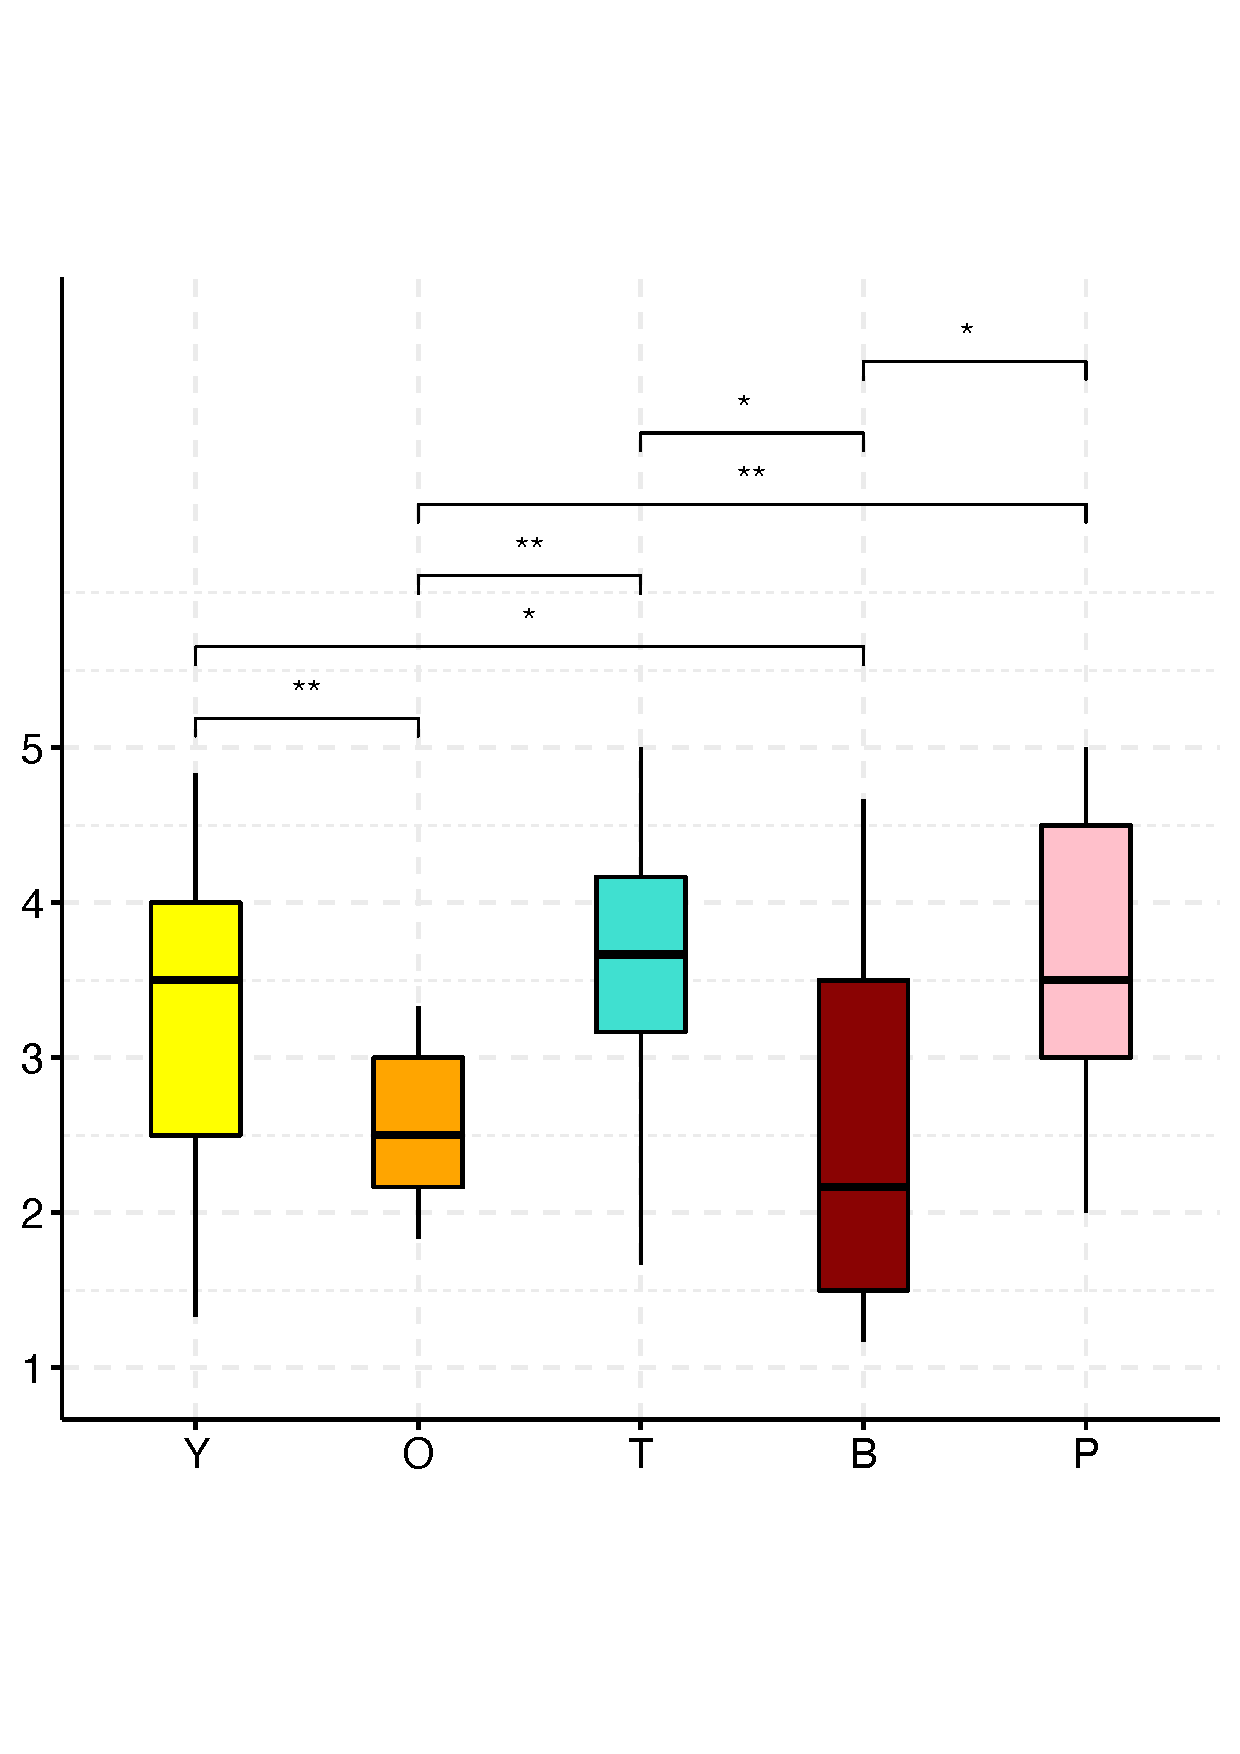
\includegraphics[width=1\linewidth]{M_L_Study_1_Consc.pdf}
        \caption{Conscientiousness}
        \label{fig:sub1}
    \end{subfigure}\hfill%
    \begin{subfigure}{.45\textwidth}
        \centering
        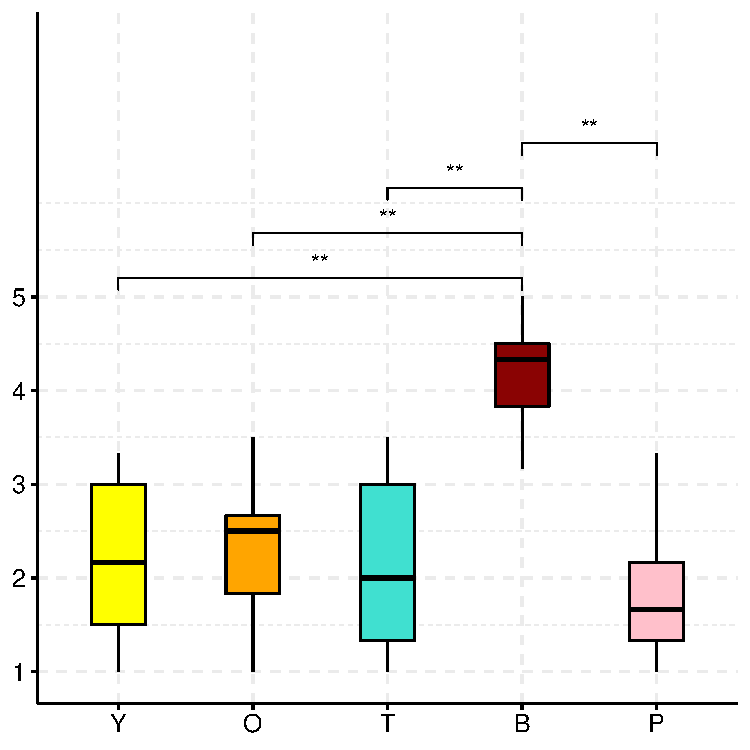
\includegraphics[width=1\linewidth]{M_L_Study_1_Neurot.pdf}
        \caption{Neuroticism}
        \label{fig:sub1}
    \end{subfigure}\hfill%
    \begin{subfigure}{.45\textwidth}
        \centering
        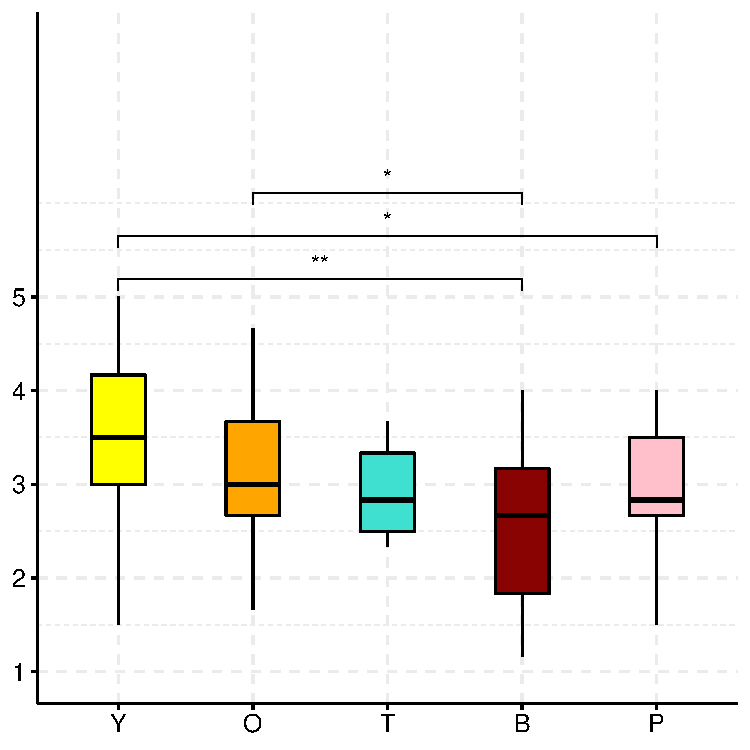
\includegraphics[width=1\linewidth]{M_L_Study_1_Open.pdf}
        \caption{Openness}
        \label{fig:sub1}
    \end{subfigure}\hfill%
    \caption{A boxplot for the mascot-lamp interaction in study-1.
    Stars represent the significance of p\textsubscript{adj} after Bonferroni correction.}
    \label{fig:ML1}
\end{figure}
%%%%%%%%%%%%%%%%%%%%%%%%%%%%%%%%%%%%%%%%%%%%%%%%%%%%%%%%%%%%%%%%%%%
\subsection{The analysis of the within lighting color study.}
\label{subsec:MLstudy2}
The second study considers the effect of the lighting color on how each
personality trait is assessed within one color condition.
Compared groups are five personality traits such as extraversion, agreeableness, conscientiousness,
neuroticism, and openness.

\par\textbf{Yellow.}
The Friedman test shows a significant difference in the ratings of each personality trait
within yellow lighting color with p<.01, df=4 (see Table~\ref{table:friedmanML2}).
When mascot triggers yellow light, the difference is concentrated on neuroticism
which is rated very low compared to other personality traits.
According to Figure~\ref{fig:ML2}, 80\% of scores given for extraversion, agreeableness,
conscientiousness, and openness are higher than all scores given for neurotic personality.
Also, the similarity of the median values for all personality traits except
neuroticism (med = 3.7, med = 3.7, med = 3.5, med = 3.5) reveals a small effect of yellow
color on these four personality traits (see Table~\ref{table:medianML2}).

\par\textbf{Orange.}
There is a statistically substantial difference between personality trait measurements within
orange color with p<.01, df=4 (see Table~\ref{table:friedmanML2}).
When orange color is triggered, the mascot with extraversion and openness traits
show distinguishable ratings in comparison to all other personalities with p<.05 (see Figure~\ref{fig:ML2}).
Moreover, tests did not show any significant differences between extraversion (med = 3.0, max = 4.8, min = 2.3)
and openness (med = 3.0, max = 4.7, min = 1.7) within orange color (see Table~\ref{table:medianML2}).
However, the median values of extraversion and openness are higher compared to the
values of all other personality traits.

\par\textbf{Turquoise.}
Overall, all personality traits are measured differently when the light was transformed to turquoise color
with p<0.01, df=4 (see Table~\ref{table:friedmanML2}).
Wilcoxon test reveals that when the turquoise is displayed, the agreeableness and conscientiousness
personality traits are substantially distinguishable from other personality traits with p<.05 (see Figure~\ref{fig:ML2}).
Both of them are measured high when mascot triggers turquoise color.
However, these two personalities are not distinguishable from each other within turquoise color.
In spite of that fact, the median value of conscientiousness (med = 3.7) is slightly higher than
for agreeableness (med = 3.5) (see Table~\ref{table:medianML2}).

\par\textbf{Blood-red}
lighting color reveals a significant difference in measurements of all personality traits
with p<.01, df=4 (see Table~\ref{table:friedmanML2}).
According to Figure~\ref{fig:ML2}, there is an excellent separation of neuroticism boxplot from all other personality traits.
Table~\ref{table:medianML2} shows a very high median value for neuroticism compared to other
personality traits with med = 4.3, max = 5.0 and min = 3.2.

\par\textbf{Pink.}
There is a significant difference in ratings of the mascots' personality when the pink light is
triggered having p<.01, df=4 (see Table~\ref{table:friedmanML2}).
According to Figure~\ref{fig:ML2}, pink light shows a significant effect on the agreeableness
and conscientiousness with p\textsubscript{adj}<.01 comparing to extraversion, neuroticism, and openness personality traits.
Based on the medians reported in Table~\ref{table:medianML2}, agreeableness has the
highest (med = 4.0) in contrast to neuroticism which has the lowest value (med = 1.7).

\begin{table}[hbt!]
    \renewcommand{\arraystretch}{1}
    \begin{center}
        \begin{tabular}{|c|c|c|c|}
            \hline
            \textbf{Color conditions} & \textbf{$\chi^2$} & \textbf{df} & \textbf{p} \\
            \hline
            Yellow &23.6 &4 &p<.01 \\
            \hline
            Orange &38.2 &4 &p<.01\\
            \hline
            Turquoise &37.1 &4 &p<.01 \\
            \hline
            Blood-red &45.5 &4 &p<.01 \\
            \hline
            Pink &60.1 &4 &p<.01 \\
            \hline
        \end{tabular}
        \caption{The results of the Friedman test for five color conditions in the case of mascot-lamp interaction.}
        \label{table:friedmanML2}
    \end{center}
\end{table}

\begin{table}[hbt!]
    \renewcommand{\arraystretch}{1}
    \begin{center}
        \begin{tabular}{p{0.05\textwidth}|
        p{0.025\textwidth}|p{0.025\textwidth}|p{0.025\textwidth}|p{0.025\textwidth}|p{0.025\textwidth}||
        p{0.025\textwidth}|p{0.025\textwidth}|p{0.025\textwidth}|p{0.025\textwidth}|p{0.025\textwidth}||
        p{0.025\textwidth}|p{0.025\textwidth}|p{0.025\textwidth}|p{0.025\textwidth}|p{0.025\textwidth}|}
            \cline{2-16}
            & \multicolumn{5}{c||}{\textbf{Yellow}} & \multicolumn{5}{c||}{\textbf{Orange}}
            & \multicolumn{5}{c|}{\textbf{Turquoise}} \\
            \cline{2-16}
            & E & A & C & N & O & E & A & C & N & O & E & A & C & N & O      \\
            \cline{2-16}
            \textbf{Min}    & 2.3 & 1.8 & 1.3 & 1.0 & 1.5 & 2.3 & 1.0 & 1.8 & 1.0 & 1.7 & 1.8 & 2.0 & 1.7 & 1.0 & 2.3  \\
            \textbf{Med}    & 3.7 & 3.7 & 3.5 & 2.2 & 3.5 & 3.0 & 2.3 & 2.5 & 2.5 & 3.0 & 2.7 & 3.5 & 3.7 & 2.0 & 2.8  \\
            \textbf{Max}    & 4.8 & 5.0 & 4.8 & 3.3 & 5.0 & 4.8 & 3.3 & 3.3 & 3.5 & 4.7 & 4.2 & 5.0 & 5.0 & 3.5 & 3.7 \\
            \cline{2-16}
            \cline{2-11}
            &  \multicolumn{5}{|c||}{\textbf{Blood-red}} & \multicolumn{5}{|c||}{\textbf{Pink}} \\
            \cline{2-11}
            & E & A & C & N & O & E & A & C & N & O            \\
            \cline{2-11}
            \textbf{Min}    & 1.0 & 1.0 & 1.2 & 3.2 & 1.2 & 1.7 & 2.5 & 2.0 & 1.0 & 1.5    \\
            \textbf{Med}    & 1.7 & 2.0 & 2.2 & 4.3 & 2.7 & 2.8 & 4.0 & 3.5 & 1.7 & 2.8    \\
            \textbf{Max}    & 4.5 & 3.8 & 4.7 & 5.0 & 4.0 & 3.7 & 5.0 & 5.0 & 3.3 & 4.0    \\
            \cline{2-11}
        \end{tabular}
        \caption{A summary table of the median, minimum, and maximum rates given for each color condition.}
        \label{table:medianML2}
    \end{center}
\end{table}
%%%%%%%
\begin{figure}[hbt!]
    \centering
    \begin{subfigure}{.45\textwidth}
        \centering
        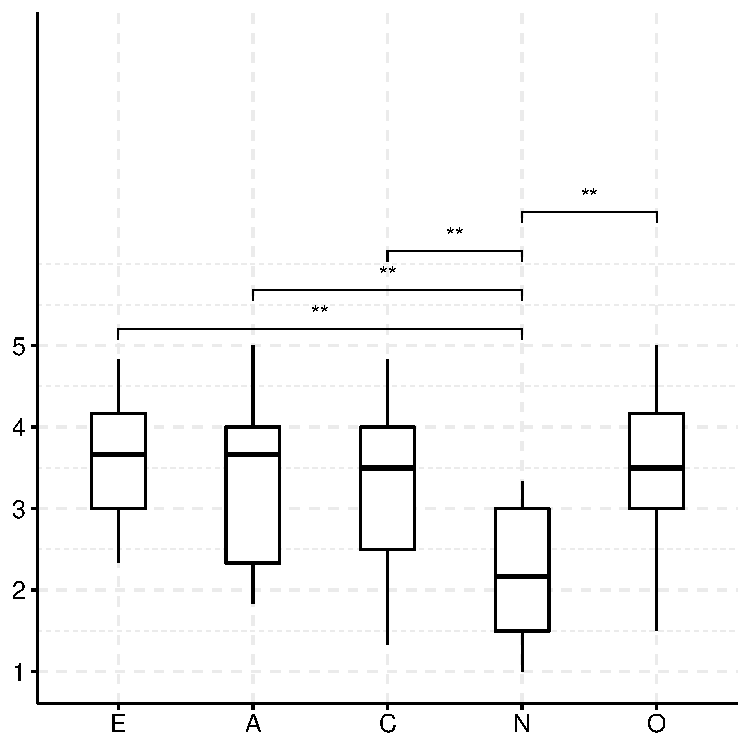
\includegraphics[width=1\linewidth]{M_L_Study_2_Yel.pdf}
        \caption{Yellow}
        \label{fig:sub1}
    \end{subfigure}\hfill%
    \begin{subfigure}{.45\textwidth}
        \centering
        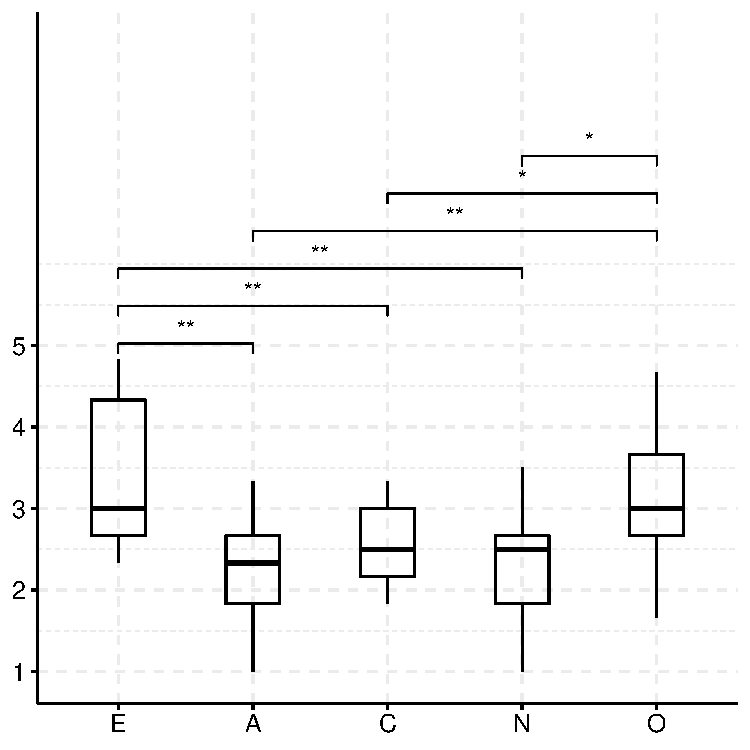
\includegraphics[width=1\linewidth]{M_L_Study_2_Oran.pdf}
        \caption{Orange}
        \label{fig:sub2}
    \end{subfigure}\hfill
    \begin{subfigure}{.45\textwidth}
        \centering
        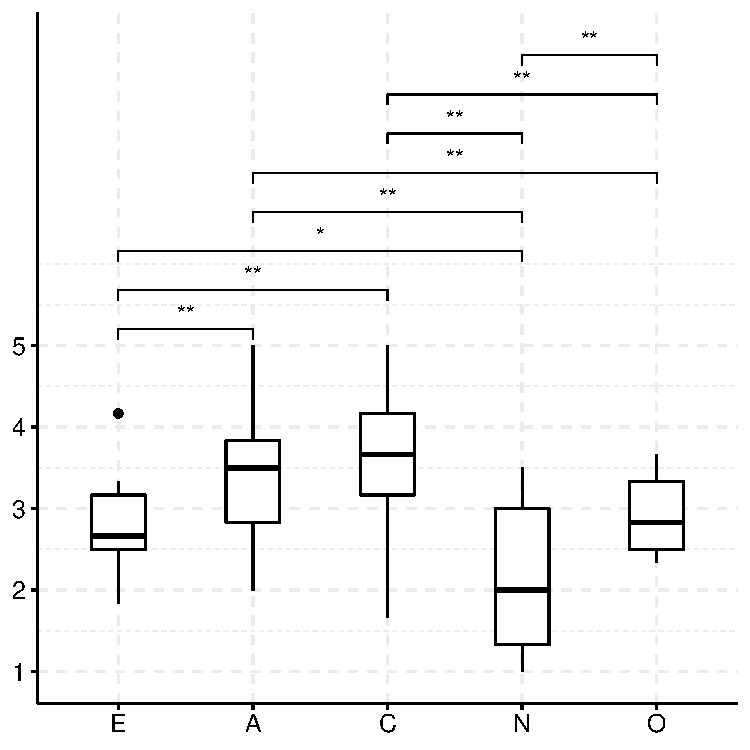
\includegraphics[width=1\linewidth]{M_L_Study_2_Turq.pdf}
        \caption{Turquoise}
        \label{fig:sub1}
    \end{subfigure}\hfill%
    \begin{subfigure}{.45\textwidth}
        \centering
        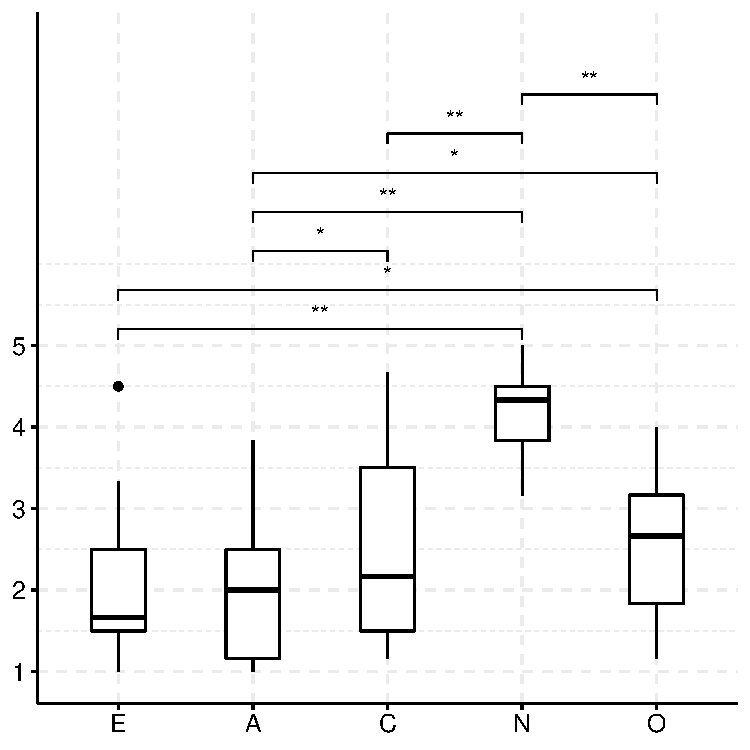
\includegraphics[width=1\linewidth]{M_L_Study_2_Blr.pdf}
        \caption{Blood-red}
        \label{fig:sub1}
    \end{subfigure}\hfill%
    \begin{subfigure}{.45\textwidth}
        \centering
        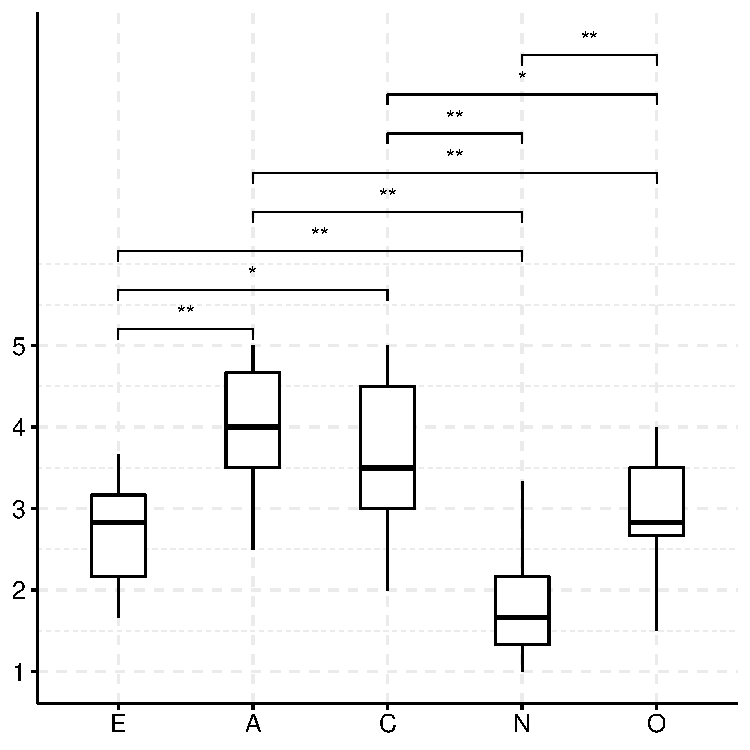
\includegraphics[width=1\linewidth]{M_L_Study_2_Pin.pdf}
        \caption{Pink}
        \label{fig:sub1}
    \end{subfigure}\hfill%
    \caption{A boxplot for the mascot-lamp interaction in study-2.
    Stars represent the significance of p\textsubscript{adj} after Bonferroni correction.}
    \label{fig:ML2}
\end{figure}
%%%%%%%%%%%%%%%%%%%%%%%%%%%%%%%%%%%%%%%%%%%%%%%%%%%%%%%%%%%%%%%%%%%%%%%%%%%%%%%%%%%%%%%%%%%%%%%%%%%%%%%%%%%%%%%%%%%%%%%%
\section{The analysis of the mascot-mascot interaction.}
\label{sec:m-m}
This section covers the analysis of the effect of each level of vibration on the perception
of the personality trait of approaching mascot which triggers this vibration.
In Subsection~\ref{subsec:MMstudy1}, the statistical tests are conducted for the within
personality trait study and in Subsection~\ref{subsec:MMstudy2} for the within vibration level.
Besides, from now on each vibration level is abbreviated accordingly.
For example, the vibration with 500-millisecond duration is abbreviated
as ‘level-5’, and with 100-millisecond long as ‘level-1’ and so on.

%%%%%%%%%%%%%%%%%%%%%%%%%%%%%%%%%%%%%%%%%%%%%%%%%%%%%%%%%%%%%%%%%%%
\subsection{The analysis of the within personality trait study.}
\label{subsec:MMstudy1}
In the first study, compared factors are five levels of vibration starting from level-1 to level-5.

\par\textbf{Extraversion.}
The Friedman test shows a significant difference between all levels of vibration in the
ratings of an extraversion personality trait with p<.01 (see Table~\ref{table:friedmanMM1}).
In comparison to all other levels, level-5 and level-4 show a significant difference
in the measurements of the extraversion personality with p<.05 (see Figure~\ref{fig:MM1}).
Both of these levels are highly scored as the behavior of an extravert mascot
with med = 4.0 for level-5 and med = 3.0 for level-4 (see Table~\ref{table:medianMM1}).

\par\textbf{Agreeableness.}
All vibration levels substantially affects the measurements of an agreeableness personality
trait with p<.01, df=4 (see Table~\ref{table:friedmanMM1}).
Both level-2 and level-3 revealed a significant effect for mascot being
assessed as agreeable with p\textsubscript{adj}<.05 (see Figure~\ref{fig:MM1}).
Overall, the majority of votes given for level-2 (med = 4.0, max = 4.7, min = 2.0) and level-3
(med = 3.5, max = 5.0, min = 2.5) are higher than most
votes given for other vibration levels (see Table~\ref{table:medianMM1}).

\par\textbf{Conscientiousness.}
There is a significant impact of all vibration levels on the assessment of conscientiousness
personality trait with p<.01, df=4 (see Table~\ref{table:friedmanMM1}).
The analysis revealed a strong difference of levels three and four
from scores given for other vibrations with p\textsubscript{adj}<.01 (see Figure~\ref{fig:MM1}).
Moreover, the median values for level-3 (med = 3.8) and level-4 (med = 4.0) are high enough
to show a strong impact of these levels to measure mascot as conscientious (see Table~\ref{table:medianMM1}).

\par\textbf{Neuroticism.}
There is a significant difference in measurements of each level of vibration within neuroticism
personality trait with p<.01, df=4 (see Table~\ref{table:friedmanMM1}).
Especially, this difference is concentrated on the ratings for level-1 with med = 3.7
in comparison to other levels having med < 2.5 (see Table~\ref{table:medianMM1}).
According to Figure~\ref{fig:MM1}, for a neuroticism personality trait, there is a good separation of samples for level-1
from all other vibration levels with p\textsubscript{adj}<.05.

\par\textbf{Openness.}
Table~\ref{table:friedmanMM1} reveals a difference between all five vibration levels within
openness personality trait with p<.05, df=4 (see Table~\ref{table:friedmanMM1}).
The Wilcoxon test revealed a significant difference between levels one and two,
during the measurements of the openness personality trait with p<.05 (see Figure~\ref{fig:MM1}).
The median values for levels five, four, two, and one imply the overall
similarity of votes concentrated on the 'neutral' scale with med < 2.7 (see Table~\ref{table:medianMM1}).

\begin{table}[hbt!]
    \renewcommand{\arraystretch}{1}
    \begin{center}
        \begin{tabular}{|c|c|c|c|}
            \hline
            \textbf{Personality traits} & \textbf{$\chi^2$} & \textbf{df} & \textbf{p} \\
            \hline
            Extraversion &30.8 &4 &p<.01 \\
            \hline
            Agreeableness &19.8 &4 &p<.01 \\
            \hline
            Conscientiousness & 43.2 &4 &p<.01 \\
            \hline
            Neuroticism &28.2 &4 &p<.01\\
            \hline
            Openness &11.2 &4 &p<.05 \\
            \hline
        \end{tabular}
        \caption{The results of the Friedman test for all personality traits in the case of mascot-mascot interaction.}
        \label{table:friedmanMM1}
    \end{center}
\end{table}

\begin{table}[hbt!]
    \renewcommand{\arraystretch}{1}
    \begin{center}
        \begin{tabular}{p{0.05\textwidth}|
        p{0.025\textwidth}|p{0.025\textwidth}|p{0.025\textwidth}|p{0.025\textwidth}|p{0.025\textwidth}||
        p{0.025\textwidth}|p{0.025\textwidth}|p{0.025\textwidth}|p{0.025\textwidth}|p{0.025\textwidth}||
        p{0.025\textwidth}|p{0.025\textwidth}|p{0.025\textwidth}|p{0.025\textwidth}|p{0.025\textwidth}|}
            \cline{2-16}
            & \multicolumn{5}{c||}{\textbf{Extraversion}} & \multicolumn{5}{c||}{\textbf{Agreeableness}}
            & \multicolumn{5}{c|}{\textbf{Conscientiousness}} \\
            \cline{2-16}
            & L1 & L2 & L3 & L4 & L5 & L1 & L2 & L3 & L4 & L5 & L1 & L2 & L3 & L4 & L5      \\
            \cline{2-16}
            \textbf{Min}    & 1.2 & 1.7 & 1.3 & 2.2 & 2.3 & 1.7 & 2.0 & 2.5 & 1.3 & 1.3 & 1.7 & 1.5 & 2.8 & 2.2 & 1.7  \\
            \textbf{Med}    & 2.0 & 2.0 & 2.7 & 3.0 & 4.0 & 2.5 & 4.0 & 3.5 & 2.8 & 2.7 & 2.5 & 2.7 & 3.8 & 4.0 & 2.8  \\
            \textbf{Max}    & 3.8 & 4.0 & 4.3 & 4.7 & 4.7 & 4.0 & 4.7 & 5.0 & 4.0 & 3.8 & 3.8 & 4.2 & 5.0 & 5.0 & 3.8 \\
            \cline{2-16}
            \cline{2-11}
            &  \multicolumn{5}{|c||}{\textbf{Neuroticism}} & \multicolumn{5}{|c||}{\textbf{Openness}} \\
            \cline{2-11}
            & L1 & L2 & L3 & L4 & L5 & L1 & L2 & L3 & L4 & L5            \\
            \cline{2-11}
            \textbf{Min}    & 2.0 & 1.3 & 1.3 & 1.0 & 1.0 & 1.1 & 1.8 & 1.5 & 1.0 & 1.3    \\
            \textbf{Med}    & 3.7 & 2.1 & 1.8 & 2.2 & 2.3 & 2.3 & 2.5 & 3.3 & 2.7 & 2.7    \\
            \textbf{Max}    & 4.7 & 3.7 & 4.2 & 3.5 & 3.3 & 4.2 & 4.5 & 4.3 & 4.5 & 4.0    \\
            \cline{2-11}
        \end{tabular}
        \caption{A summary table of the median, minimum, and maximum rates given for each personality trait.}
        \label{table:medianMM1}
    \end{center}
\end{table}

\begin{figure}[hbt!]
    \centering
    \begin{subfigure}{.45\textwidth}
        \centering
        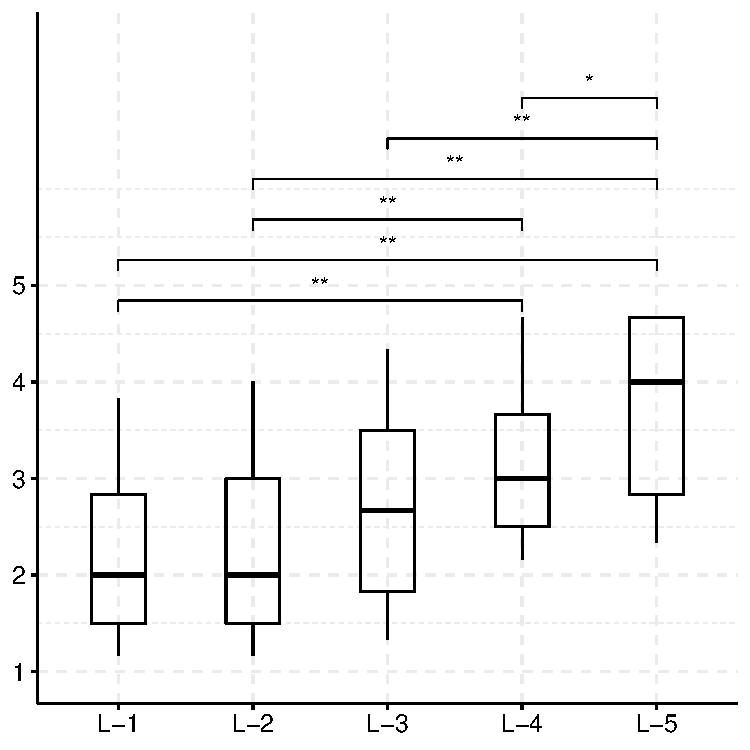
\includegraphics[width=1\linewidth]{M_M_Study_1_Extrav.pdf}
        \caption{Extraversion}
        \label{fig:sub1}
    \end{subfigure}\hfill%
    \begin{subfigure}{.45\textwidth}
        \centering
        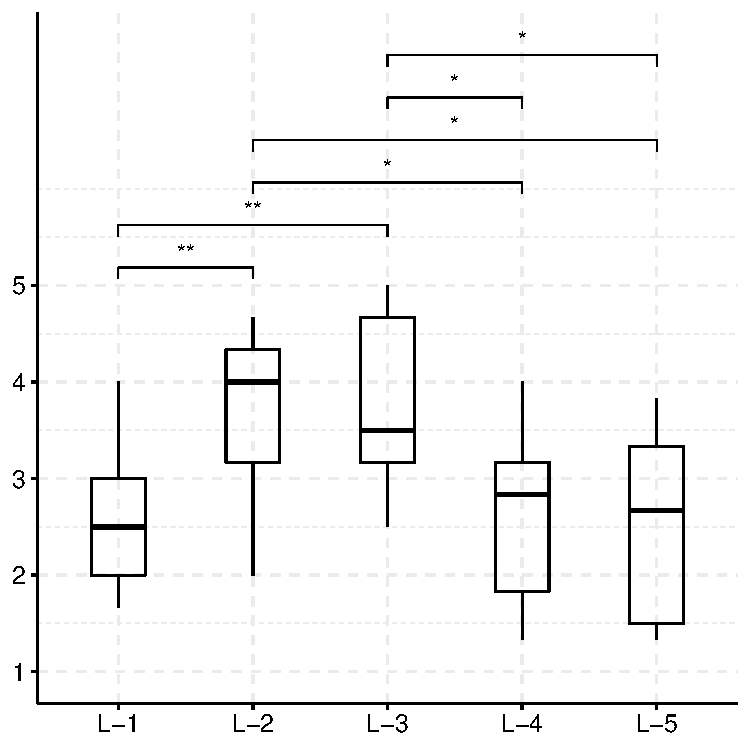
\includegraphics[width=1\linewidth]{M_M_Study_1_Agreeab.pdf}
        \caption{Agreeableness}
        \label{fig:sub2}
    \end{subfigure}\hfill
    \begin{subfigure}{.45\textwidth}
        \centering
        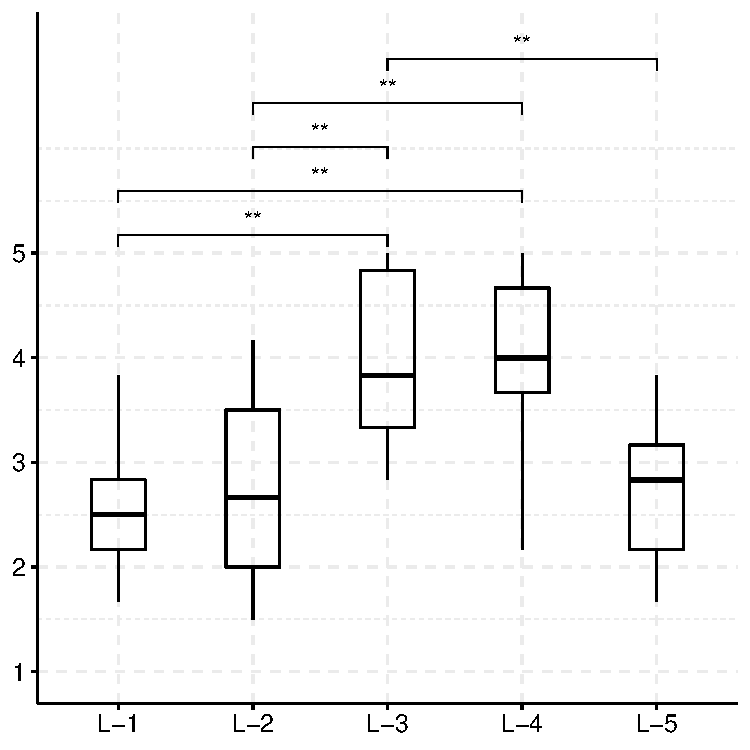
\includegraphics[width=1\linewidth]{M_M_Study_1_Consc.pdf}
        \caption{Conscientiousness}
        \label{fig:sub1}
    \end{subfigure}\hfill%
    \begin{subfigure}{.45\textwidth}
        \centering
        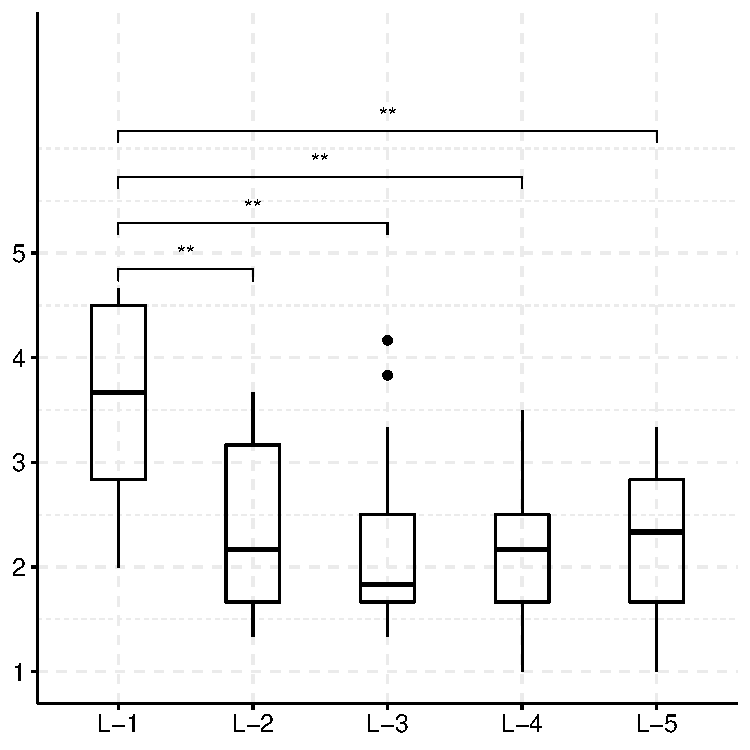
\includegraphics[width=1\linewidth]{M_M_Study_1_Neurot.pdf}
        \caption{Neuroticism}
        \label{fig:sub1}
    \end{subfigure}\hfill%
    \begin{subfigure}{.45\textwidth}
        \centering
        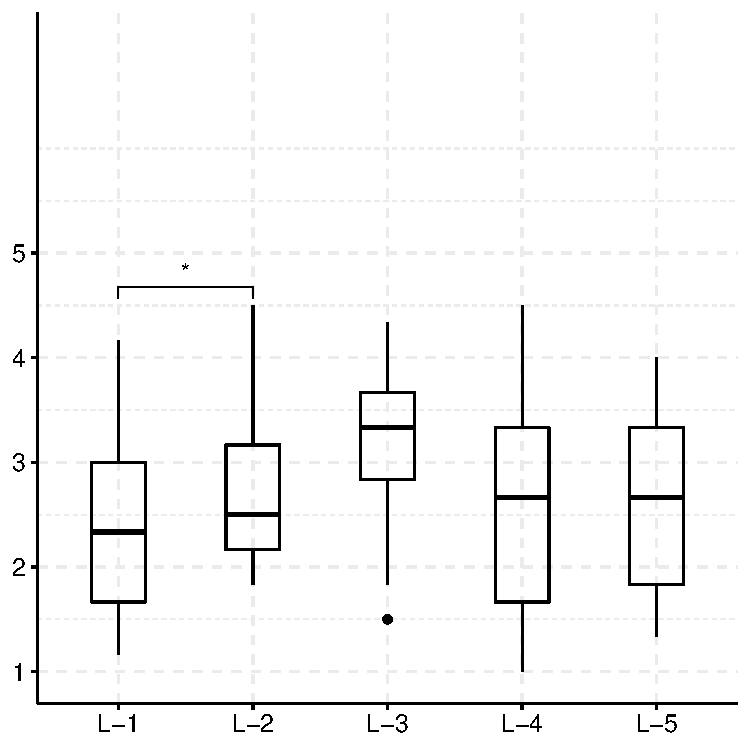
\includegraphics[width=1\linewidth]{M_M_Study_1_Open.pdf}
        \caption{Openness}
        \label{fig:sub1}
    \end{subfigure}\hfill%
    \caption{A boxplot for the mascot-mascot interaction in study-1.
    Stars represent the significance of p\textsubscript{adj} after Bonferroni correction.}
    \label{fig:MM1}
\end{figure}
%%%%%%%%%%%%%%%%%%%%%%%%%%%%%%%%%%%%%%%%%%%%%%%%%%%%%%%%%%%%%%%%%%%
\subsection{The analysis of the within vibration level study.}
\label{subsec:MMstudy2}
The second study analyzes each vibration level individually and the difference
of each personality trait within a specific vibration level.
Compared groups are extraversion, agreeableness, conscientiousness, neuroticism, and openness personality traits.

\par\textbf{Level-1.}
The Friedman test shows a significant difference between the ratings of all personality traits
and vibration level one with p<.01, df=4 (see Table~\ref{table:friedmanMM2}).
This difference especially is concentrated on neuroticism which distinguished it from all
other personality traits with p\textsubscript{adj}<.05 (see Figure~\ref{fig:MM2}).
In comparison to neuroticism (med = 3.7), the median rates given for extraversion,
agreeableness, conscientiousness, and openness personality traits are relatively similar
being 2.0, 2.5, 2.5, 2.3 respectively (see Table~\ref{table:medianMM2}).

\par\textbf{Level-2.}
On average, level-2 has a significant effect on the ratings of all five personality
traits with p<.01, df=4 (see Table~\ref{table:friedmanMM2}).
Based on Wilcoxon tests, there are four groups of personality traits being effected by
vibration level-2 with p\textsubscript{adj}<.05 (see Figure~\ref{fig:MM2}).
Agreeableness is the most distinguishable being rated higher (med = 4.0)
than all other personality traits (med < 2.8) (see Table~\ref{table:medianMM2}).

\par\textbf{Level-3}
has a substantial impact on the measurements of a personality trait
with p<.01, df=4 (see Table~\ref{table:friedmanMM2}).
Level-3 effects the ratings of two personality traits: agreeableness and
conscientiousness with p\textsubscript{adj}<.05 (see Figure~\ref{fig:MM2}).

\par\textbf{Level-4.}
There is a statistically significant difference between the measurements of all personality traits
within level-4 with p<.01, df=4 (see Table~\ref{table:friedmanMM2}).
Level-4 has an impact on the ratings of two personality traits with the highest scores (max = 4.7 and max = 5.0)
such as conscientiousness and extraversion
with a very significant p\textsubscript{adj}<.01 (see Figure~\ref{fig:MM2}).

\par\textbf{Level-5.}
Overall, all personality traits show different results when each mascot vibrating 500 milliseconds
per time (i.e.\ level-5) with p<.01, df=4 (see Table~\ref{table:friedmanMM2}).
Level-5 distinguishes extraversion from all other personality traits having the
highest ratings with p\textsubscript{adj}<.05 (see Figure~\ref{fig:MM2}).
The median values for all other personality traits are lower than the neutral scale (med < 3.0)
in comparison to neuroticism with med = 4.0 (see Table~\ref{table:medianMM2}).

\begin{table}[hbt!]
    \renewcommand{\arraystretch}{1}
    \begin{center}
        \begin{tabular}{|c|c|c|c|}
            \hline
            \textbf{Vibration levels} & \textbf{$\chi^2$} & \textbf{df} & \textbf{p} \\
            \hline
            Level-1 &24.0 &4 &p<.01 \\
            \hline
            Level-2 &24.5 &4 &p<.01 \\
            \hline
            Level-3 &35.2 &4 &p<.01 \\
            \hline
            Level-4 &46.6 &4 &p<.01 \\
            \hline
            Level-5 &24.1 &4 &p<.01 \\
            \hline
        \end{tabular}
        \caption{The results of the Friedman test for all vibration levels in the case of mascot-mascot interaction.}
        \label{table:friedmanMM2}
    \end{center}
\end{table}

\begin{table}[hbt!]
    \renewcommand{\arraystretch}{1}
    \begin{center}
        \begin{tabular}{p{0.05\textwidth}|
        p{0.025\textwidth}|p{0.025\textwidth}|p{0.025\textwidth}|p{0.025\textwidth}|p{0.025\textwidth}||
        p{0.025\textwidth}|p{0.025\textwidth}|p{0.025\textwidth}|p{0.025\textwidth}|p{0.025\textwidth}||
        p{0.025\textwidth}|p{0.025\textwidth}|p{0.025\textwidth}|p{0.025\textwidth}|p{0.025\textwidth}|}
            \cline{2-16}
            & \multicolumn{5}{c||}{\textbf{Level-1}} & \multicolumn{5}{c||}{\textbf{Level-2}}
            & \multicolumn{5}{c|}{\textbf{Level-3}} \\
            \cline{2-16}
            & E & A & C & N & O & E & A & C & N & O & E & A & C & N & O      \\
            \cline{2-16}
            \textbf{Min}    & 1.2 & 1.7 & 1.7 & 2.0 & 1.2 & 1.2 & 2.0 & 1.5 & 1.3 & 1.8 & 1.3 & 2.5 & 2.8 & 1.3 & 1.5  \\
            \textbf{Med}    & 2.0 & 2.5 & 2.5 & 3.7 & 2.3 & 2.0 & 4.0 & 2.7 & 2.2 & 2.5 & 2.7 & 3.5 & 3.8 & 1.8 & 3.3  \\
            \textbf{Max}    & 3.8 & 4.0 & 3.8 & 4.7 & 4.2 & 4.0 & 4.7 & 4.2 & 3.7 & 4.5 & 4.3 & 5.0 & 5.0 & 4.2 & 4.3 \\
            \cline{2-16}
            \cline{2-11}
            &  \multicolumn{5}{|c||}{\textbf{Level-4}} & \multicolumn{5}{|c||}{\textbf{Level-5}} \\
            \cline{2-11}
            & E & A & C & N & O & E & A & C & N & O            \\
            \cline{2-11}
            \textbf{Min}    & 2.2 & 1.3 & 2.2 & 1.0 & 1.0 & 2.3 & 1.3 & 1.7 & 1.0 & 1.3    \\
            \textbf{Med}    & 3.0 & 2.8 & 4.0 & 2.2 & 2.7 & 4.0 & 2.7 & 2.8 & 2.3 & 2.7    \\
            \textbf{Max}    & 4.7 & 4.0 & 5.0 & 3.5 & 4.5 & 4.7 & 3.8 & 3.8 & 3.3 & 4.0    \\
            \cline{2-11}
        \end{tabular}
        \caption{A summary table of the median, minimum, and maximum rates given for each vibration level.}
        \label{table:medianMM2}
    \end{center}
\end{table}

\begin{figure}[hbt!]
    \centering
    \begin{subfigure}{.45\textwidth}
        \centering
        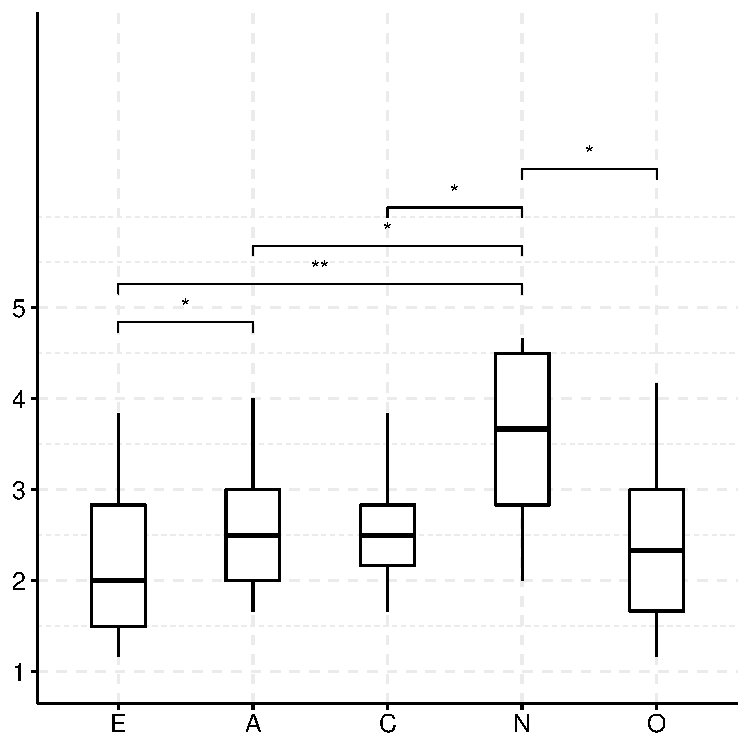
\includegraphics[width=1\linewidth]{M_M_Study_2_L1.pdf}
        \caption{Level-1}
        \label{fig:sub1}
    \end{subfigure}\hfill%
    \begin{subfigure}{.45\textwidth}
        \centering
        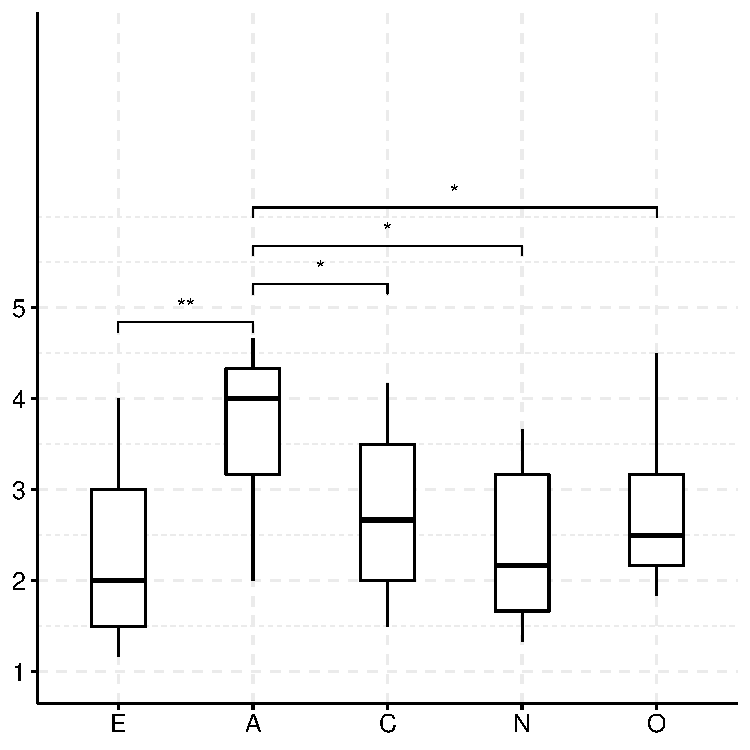
\includegraphics[width=1\linewidth]{M_M_Study_2_L2.pdf}
        \caption{Level-2}
        \label{fig:sub2}
    \end{subfigure}\hfill
    \begin{subfigure}{.45\textwidth}
        \centering
        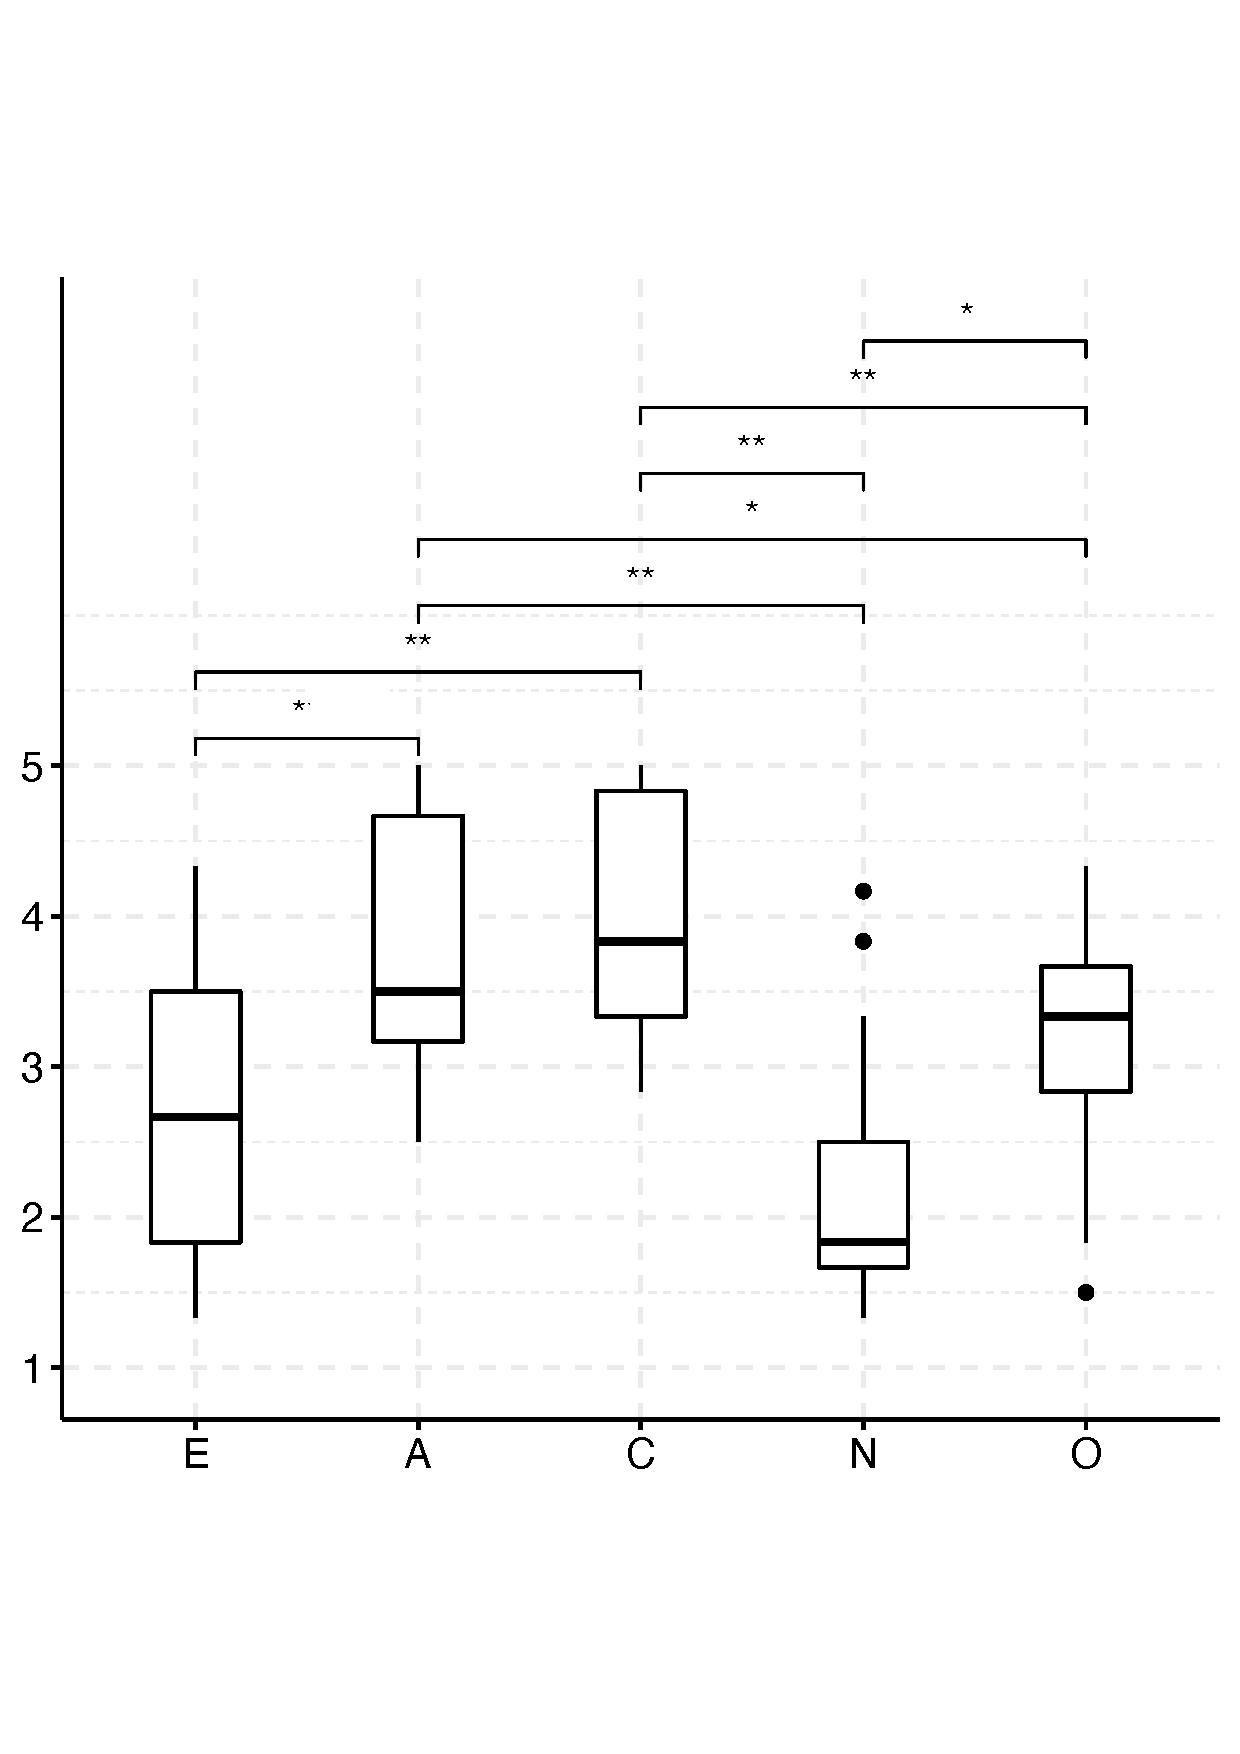
\includegraphics[width=1\linewidth]{M_M_Study_2_L3.pdf}
        \caption{Level-3}
        \label{fig:sub1}
    \end{subfigure}\hfill%
    \begin{subfigure}{.45\textwidth}
        \centering
        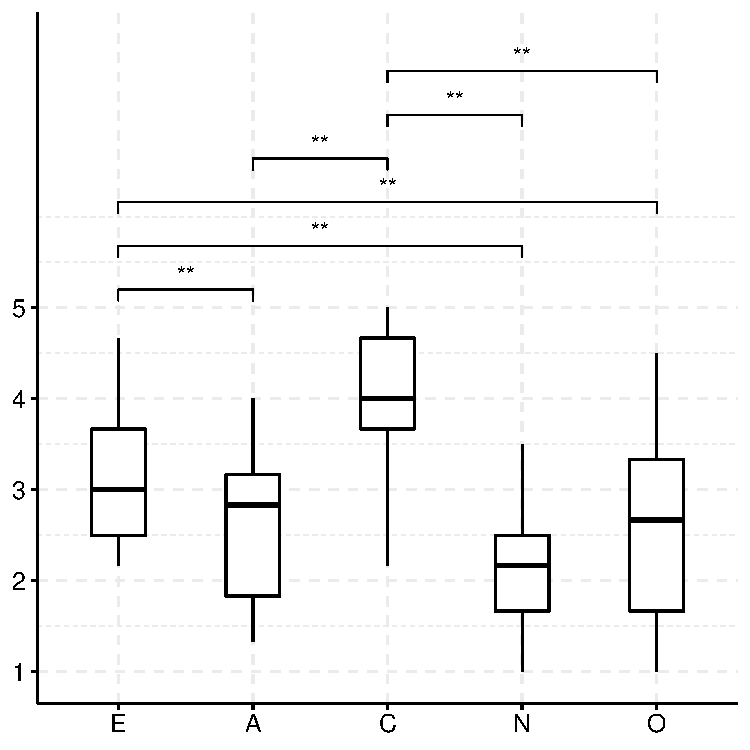
\includegraphics[width=1\linewidth]{M_M_Study_2_L4.pdf}
        \caption{Level-4}
        \label{fig:sub1}
    \end{subfigure}\hfill%
    \begin{subfigure}{.45\textwidth}
        \centering
        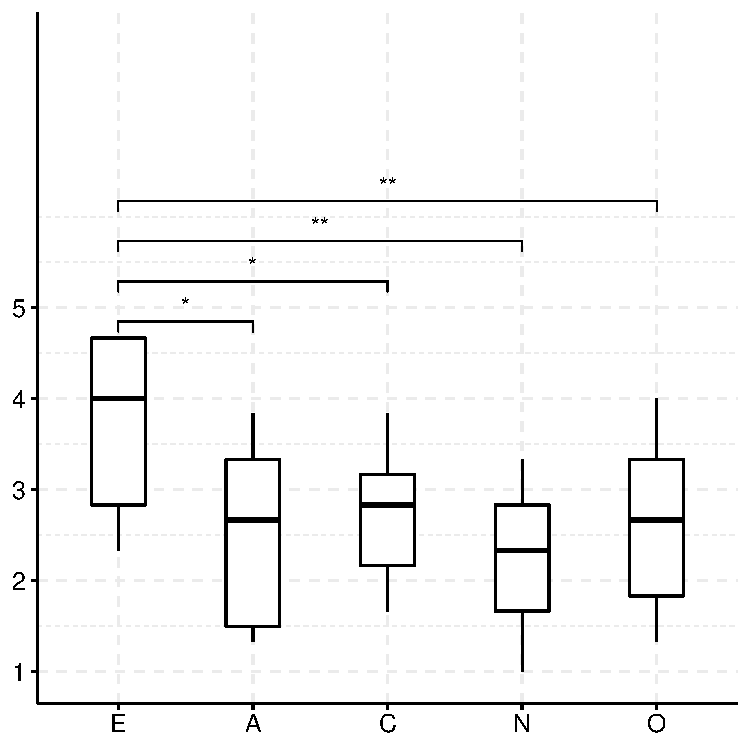
\includegraphics[width=1\linewidth]{M_M_Study_2_L5.pdf}
        \caption{Level-5}
        \label{fig:sub1}
    \end{subfigure}\hfill%
    \caption{A boxplot for the mascot-mascot interaction in study-2.
    Stars represent the significance of p\textsubscript{adj} after Bonferroni correction.}
    \label{fig:MM2}
\end{figure}
%%%%%%%%%%%%%%%%%%%%%%%%%%%%%%%%%%%%%%%%%%%%%%%%%%%%%%%%%%%%%%%%%%%%%%%%%%%%%%%%%%%%%%%%%%%%%%%%%%%%%%%%%%%%%%%%%%%%%%%%
\section{The analysis of the mascot-tablet interaction.}
\label{sec:m-t}
The section describes the impact of the screen color of a tablet on the assessment of the
personality trait that mascot conveys.
Subsection~\ref{subsec:MTstudy1} shows the analysis of the within personality study
and Subsection~\ref{subsec:MTstudy2} of within condition study (i.e.\ color).

%%%%%%%%%%%%%%%%%%%%%%%%%%%%%%%%%%%%%%%%%%%%%%%%%%%%%%%%%%%%%%%%%%%
\subsection{The analysis of the within personality trait study.}
\label{subsec:MTstudy1}
The first study is focused on each personality by comparing the scores given
for each color within that personality trait.
Compared factors are yellow, orange, turquoise, blood-red, and pink screen colors.

\par\textbf{Extraversion.}
For the measurements of extraversion personality,
the most significant difference was observed when yellow and orange was compared to
blood-red and pink colors with p\textsubscript{adj}<.05 (see Figure~\ref{fig:MT1}).
Moreover, in comparison to other colors most samples for orange are concentrated around
an 'accurate' score (med = 4.2, max = 5.0) (see Table~\ref{table:medianMT1}).

\par\textbf{Agreeableness.}
The change in tablet's screen color significantly influenced the participants' ratings of
an agreeableness personality trait with p<.01, df=4 (see Table~\ref{table:friedmanMT1}).
Figure~\ref{fig:MT1}) shows a good separation of turquoise and pink colors
from all others implying that there is a difference in ratings of the
agreeableness personality traits having p\textsubscript{adj}<.01.
However, there is no strong difference between turquoise and pink colors having
the same value med = 3.7 (see Table~\ref{table:medianMT1}).

\par\textbf{Conscientiousness.}
There is a significant difference in the rating of conscientiousness personality trait
when comparing screen colors with p<.01, df=4 (see Table~\ref{table:friedmanMT1}).
According to Figure~\ref{fig:MT1}, there is a distinguishable impact of the
tablet displaying turquoise color on the measurements of the mascot as conscientiousness with p\textsubscript{adj}<.05.
The median values for yellow (med = 2.7), pink (med = 2.8) and orange (med = 2.7) colors are
concentrated around the 'neutral' scale, whereas turquoise (med = 4.2)
is concentrated near 'accurate' scale (see Table~\ref{table:medianMT1}).

\par\textbf{Neuroticism.}
All predefined screen colors substantially affects the measurements of the neuroticism personality
trait with p<.01, df=4 (see Table~\ref{table:friedmanMT1}).
According to Figure~\ref{fig:MT1}, there is a great separation of blood-red
samples from all other screen colors with p\textsubscript{adj}<.05.
The ratings for the blood-red are higher with med = 3.8 compared to all other colors
with M $\leq$ 2.5 (see Table~\ref{table:medianMT1}).

\par\textbf{Openness.}
Table~\ref{table:friedmanMT1} shows the different effects based on all colors within openness
personality trait with p<.01, df=4 (see Table~\ref{table:friedmanMT1}).
According to the Wilcoxon tests, during the measurements of a mascot's openness to experience
personality traits, the yellow is significantly different from all other screen
colors with p\textsubscript{adj}<.05 (see Figure~\ref{fig:MT1}).
In comparison to all other colors (M $\leq$ 3.0), most of the samples of yellow color are discriminated
from all others concentrating around an 'accurate scale with a med = 4.0 (see Table~\ref{table:medianMT1}).

\begin{table}[hbt!]
    \renewcommand{\arraystretch}{1}
    \begin{center}
        \begin{tabular}{|c|c|c|c|}
            \hline
            \textbf{Personality traits} & \textbf{$\chi^2$} & \textbf{df} & \textbf{p} \\
            \hline
            Extraversion &28.8 &4 &p<.01 \\
            Agreeableness &52.9 &4 &p<.01 \\
            Conscientiousness &32.9 &4 &p<.01 \\
            Neuroticism &30.5 &4 &p<.01 \\
            Openness &37.7 &4 &p<.01 \\
            \hline
        \end{tabular}
        \caption{The results of the Friedman test for all personality traits in the case of mascot-tablet interaction.}
        \label{table:friedmanMT1}
    \end{center}
\end{table}

\begin{table}[hbt!]
    \renewcommand{\arraystretch}{1}
    \begin{center}
        \begin{tabular}{p{0.05\textwidth}|
        p{0.025\textwidth}|p{0.025\textwidth}|p{0.025\textwidth}|p{0.025\textwidth}|p{0.025\textwidth}||
        p{0.025\textwidth}|p{0.025\textwidth}|p{0.025\textwidth}|p{0.025\textwidth}|p{0.025\textwidth}||
        p{0.025\textwidth}|p{0.025\textwidth}|p{0.025\textwidth}|p{0.025\textwidth}|p{0.025\textwidth}|}
            \cline{2-16}
            & \multicolumn{5}{c||}{\textbf{Extraversion}} & \multicolumn{5}{c||}{\textbf{Agreeableness}}
            & \multicolumn{5}{c|}{\textbf{Conscientiousness}} \\
            \cline{2-16}
            & Y & O & T & B & P & Y & O & T & B & P & Y & O & T & B & P     \\
            \cline{2-16}
            \textbf{Min}    & 2.0 & 1.7 & 2.0 & 1.2 & 1.7 & 1.5 & 1.2 & 1.8 & 1.0 & 1.7 & 1.8 & 2.2 & 2.0 & 1.0 & 2.0  \\
            \textbf{Med}    & 3.3 & 4.2 & 2.8 & 1.7 & 2.5 & 3.0 & 2.3 & 3.7 & 1.8 & 3.7 & 2.7 & 2.7 & 4.2 & 2.3 & 2.8  \\
            \textbf{Max}    & 4.0 & 5.0 & 4.3 & 4.7 & 3.8 & 3.7 & 4.5 & 4.2 & 3.3 & 5.0 & 3.5 & 4.5 & 5.0 & 4.3 & 4.7 \\
            \cline{2-16}
            \cline{2-11}
            &  \multicolumn{5}{|c||}{\textbf{Neuroticism}} & \multicolumn{5}{|c||}{\textbf{Openness}} \\
            \cline{2-11}
            & Y & O & T & B & P & Y & O & T & B & P            \\
            \cline{2-11}
            \textbf{Min}    & 1.3 & 1.5 & 1.0 & 1.5 & 1.2 & 2.5 & 1.3 & 2.0 & 1.0 & 1.5    \\
            \textbf{Med}    & 2.2 & 2.5 & 2.5 & 3.8 & 2.3 & 4.0 & 3.0 & 3.0 & 2.7 & 2.7    \\
            \textbf{Max}    & 3.7 & 4.3 & 3.5 & 5.0 & 4.2 & 5.0 & 5.0 & 4.2 & 3.8 & 3.8    \\
            \cline{2-11}
        \end{tabular}
        \caption{A summary table of the median, minimum, and maximum rates given for each personality trait.}
        \label{table:medianMT1}
    \end{center}
\end{table}

\begin{figure}[hbt!]
    \centering
    \begin{subfigure}{.45\textwidth}
        \centering
        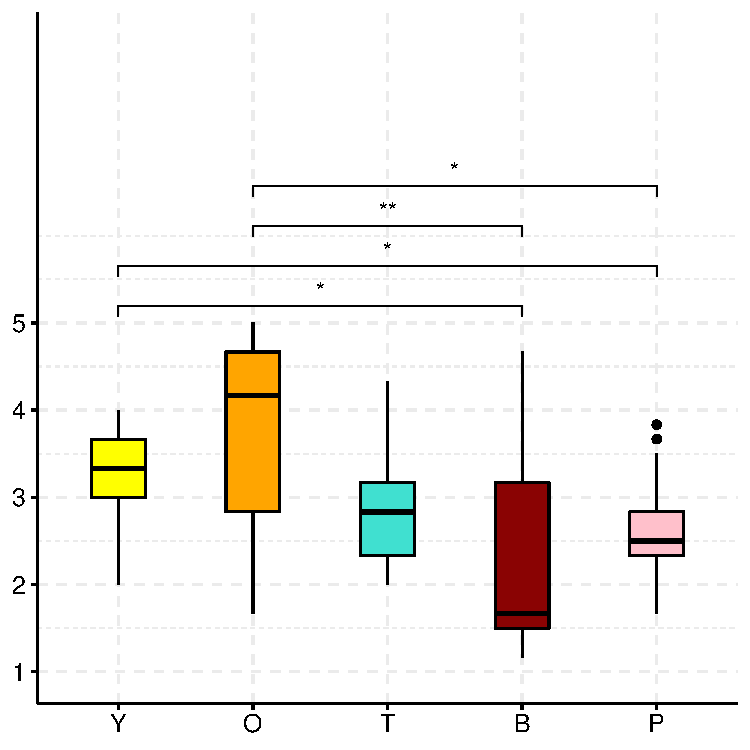
\includegraphics[width=1\linewidth]{M_T_Study_1_Extrav.pdf}
        \caption{Extraversion}
        \label{fig:sub1}
    \end{subfigure}\hfill%
    \begin{subfigure}{.45\textwidth}
        \centering
        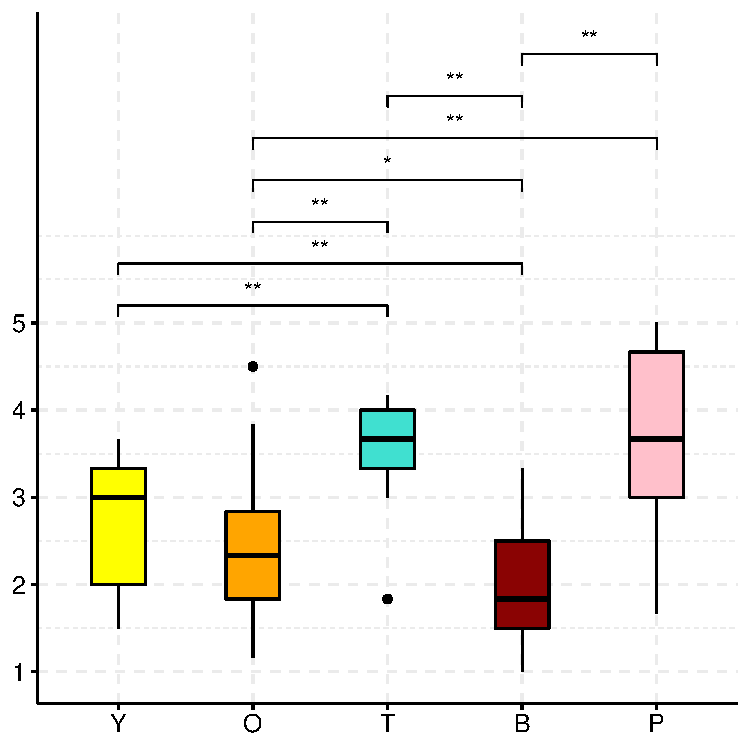
\includegraphics[width=1\linewidth]{M_T_Study_1_Agreeab.pdf}
        \caption{Agreeableness}
        \label{fig:sub2}
    \end{subfigure}\hfill
    \begin{subfigure}{.45\textwidth}
        \centering
        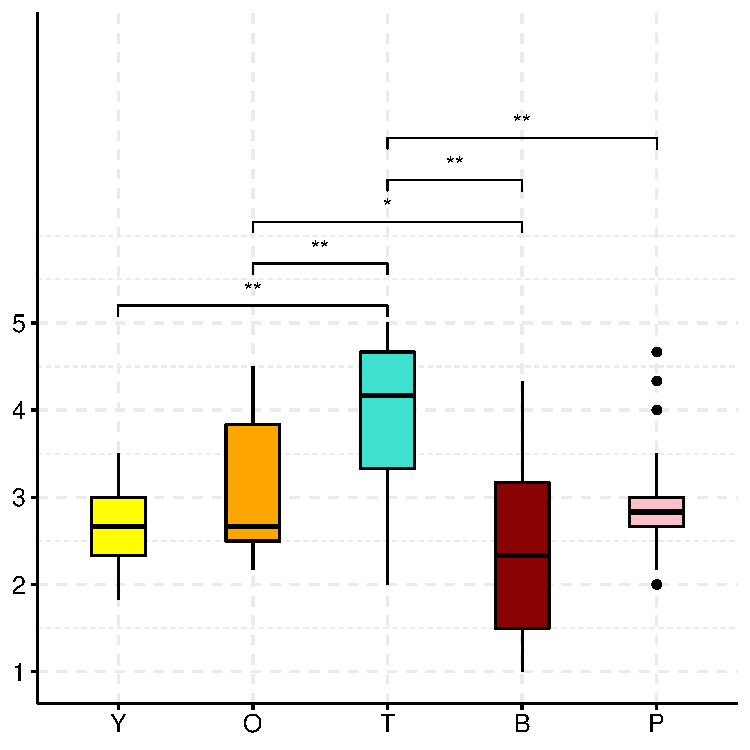
\includegraphics[width=1\linewidth]{M_T_Study_1_Consc.pdf}
        \caption{Conscientiousness}
        \label{fig:sub1}
    \end{subfigure}\hfill%
    \begin{subfigure}{.45\textwidth}
        \centering
        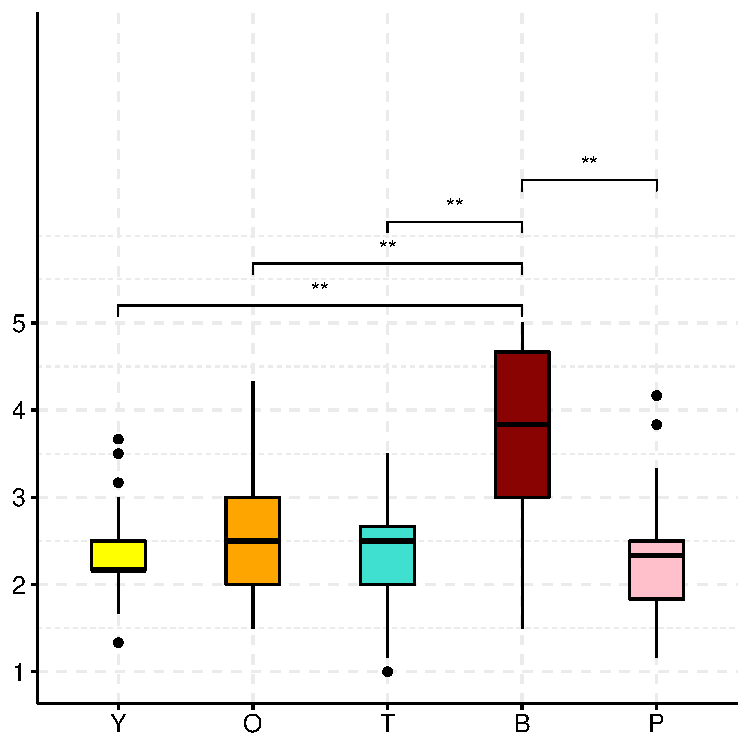
\includegraphics[width=1\linewidth]{M_T_Study_1_Neurot.pdf}
        \caption{Neuroticism}
        \label{fig:sub1}
    \end{subfigure}\hfill%
    \begin{subfigure}{.45\textwidth}
        \centering
        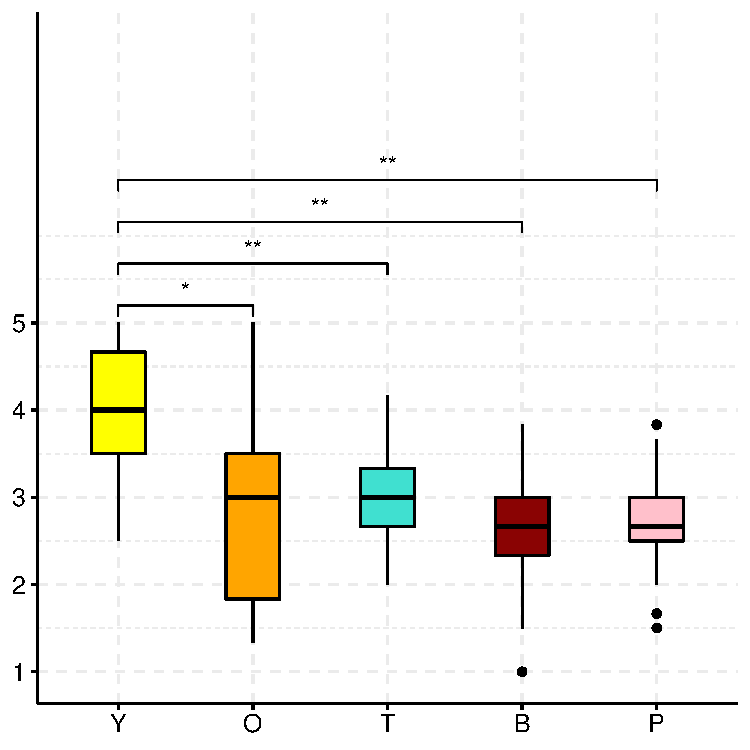
\includegraphics[width=1\linewidth]{M_T_Study_1_Open.pdf}
        \caption{Openness}
        \label{fig:sub1}
    \end{subfigure}\hfill%
    \caption{A boxplot for the mascot-tablet interaction in study-1.
    Stars represent the significance of p\textsubscript{adj} after Bonferroni correction.}
    \label{fig:MT1}
\end{figure}
%%%%%%%%%%%%%%%%%%%%%%%%%%%%%%%%%%%%%%%%%%%%%%%%%%%%%%%%%%%%%%%%%%%
\subsection{The analysis of the within screen color study.}
\label{subsec:MTstudy2}
The second study is focused on each color by comparing the different measurements of five
personality traits within each screen color.
Compared groups are extraversion, agreeableness, conscientiousness, neuroticism, and openness personality traits.

\par\textbf{Yellow.}
The Friedman test showed a significant difference in the ratings each personality trait
within yellow lighting color with p<.01, df=4 (see Table~\ref{table:friedmanMT2}).
When mascot triggers yellow background color, tests reveal openness
to be rated very high with p<.01 (see Figure~\ref{fig:MT1}).

\par\textbf{Orange.}
There is a statistically substantial difference between personality trait measurements within
orange color with p<.01, df=4 (see Table~\ref{table:friedmanML2}).
The Wilcoxon tests show the following three groups having significantly different ratings when orange
color is triggered: extraversion and agreeableness;
extraversion and neuroticism;
agreeableness and conscientiousness personality traits (see Figure~\ref{fig:MT1}).
The extraversion seems to have the highest average ratings with median = 4.2 (see Appendix A.8)

\par\textbf{Turquoise.}
Overall, all personality traits show different results when the light was transformed to turquoise color
with p<.01, df=4 (see Table~\ref{table:friedmanML2}).
Particularly, the measurements of conscientiousness and agreeableness personality traits are the most
conveyed by turquoise colors with a p\textsubscript{adj}<.05 (see Table~\ref{fig:MT2}).
The median value for conscientiousness (med = 4.2) is higher than for agreeableness
(med = 3.7) and all other personality traits (med $\leq$ 3.0) (see Table~\ref{table:friedmanMT2}).

\par\textbf{Blood-red}
lighting color reveals a significant difference in the measurements of all personality traits
with p<.01, df=4 (see Table~\ref{table:friedmanML2}).
Especially, there is a significant difference in ratings of neuroticism
being higher than for all other personality traits with p\textsubscript{adj}<.01.
The box plots display a great separation of neuroticism samples from all
other personality traits (see Figure~\ref{fig:MT1}).


\par\textbf{Pink.}
There is a significant difference in the rating mascots' personality when the pink light is
triggered with p<.01, df=4 (see Table~\ref{table:friedmanML2}).
Particularly, there is a substantial impact of pink on the scores given
for agreeableness personality with p\textsubscript{adj}<.05.
However, we could not find any difference in the ratings of pink color when
we compare agreeableness and conscientiousness personality traits
(p\textsubscript{adj}>.05 see Figure~\ref{fig:MT2}).


\begin{table}[hbt!]
    \renewcommand{\arraystretch}{1}
    \begin{center}
        \begin{tabular}{|c|c|c|c|}
            \hline
            \textbf{Color conditions} & \textbf{$\chi^2$} & \textbf{df} & \textbf{p} \\
            \hline
            Yellow &38.1 &4 &p<.01 \\
            \hline
            Orange &20.0 &4 &p<.01 \\
            \hline
            Turquoise &46.2 &4 &p<.01 \\
            \hline
            Blood-Red &30.0 &4 &p<.01 \\
            \hline
            Pink &21.7 &4 &p<.01 \\
            \hline
        \end{tabular}
        \caption{The results of the Friedman test for all color conditions in the case of mascot-tablet interaction.}
        \label{table:friedmanMT2}
    \end{center}
\end{table}

\begin{table}[hbt!]
    \renewcommand{\arraystretch}{1}
    \begin{center}
        \begin{tabular}{p{0.05\textwidth}|
        p{0.025\textwidth}|p{0.025\textwidth}|p{0.025\textwidth}|p{0.025\textwidth}|p{0.025\textwidth}||
        p{0.025\textwidth}|p{0.025\textwidth}|p{0.025\textwidth}|p{0.025\textwidth}|p{0.025\textwidth}||
        p{0.025\textwidth}|p{0.025\textwidth}|p{0.025\textwidth}|p{0.025\textwidth}|p{0.025\textwidth}|}
            \cline{2-16}
            & \multicolumn{5}{c||}{\textbf{Yellow}} & \multicolumn{5}{c||}{\textbf{Orange}}
            & \multicolumn{5}{c|}{\textbf{Turquoise}} \\
            \cline{2-16}
            & E & A & C & N & O & E & A & C & N & O & E & A & C & N & O      \\
            \cline{2-16}
            \textbf{Min}    & 2.0 & 1.5 & 1.8 & 1.3 & 2.5 & 1.7 & 1.2 & 2.2 & 1.5 & 1.3 & 2.0 & 1.8 & 2.0 & 1.0 & 2.0  \\
            \textbf{Med}    & 3.3 & 3.0 & 2.7 & 2.2 & 4.0 & 4.2 & 2.3 & 2.7 & 2.5 & 3.0 & 2.8 & 3.7 & 4.2 & 2.5 & 3.0  \\
            \textbf{Max}    & 4.0 & 3.7 & 3.5 & 3.7 & 5.0 & 5.0 & 4.5 & 4.5 & 4.3 & 5.0 & 4.3 & 4.2 & 5.0 & 3.5 & 4.2 \\
            \cline{2-16}
            \cline{2-11}
            &  \multicolumn{5}{|c||}{\textbf{Blood-red}} & \multicolumn{5}{|c||}{\textbf{Pink}} \\
            \cline{2-11}
            & E & A & C & N & O & E & A & C & N & O            \\
            \cline{2-11}
            \textbf{Min}    & 1.2 & 1.0 & 1.0 & 1.5 & 1.0 & 1.7 & 1.7 & 2.0 & 1.2 & 1.5    \\
            \textbf{Med}    & 1.7 & 1.8 & 2.3 & 3.8 & 2.7 & 2.5 & 3.7 & 2.8 & 2.3 & 2.7    \\
            \textbf{Max}    & 4.7 & 3.3 & 4.3 & 5.0 & 3.8 & 3.8 & 5.0 & 4.7 & 4.2 & 3.8    \\
            \cline{2-11}
        \end{tabular}
        \caption{A summary table of the median, minimum, and maximum rates given for each color condition.}
        \label{table:medianMT2}
    \end{center}
\end{table}

\begin{figure}[hbt!]
    \centering
    \begin{subfigure}{.45\textwidth}
        \centering
        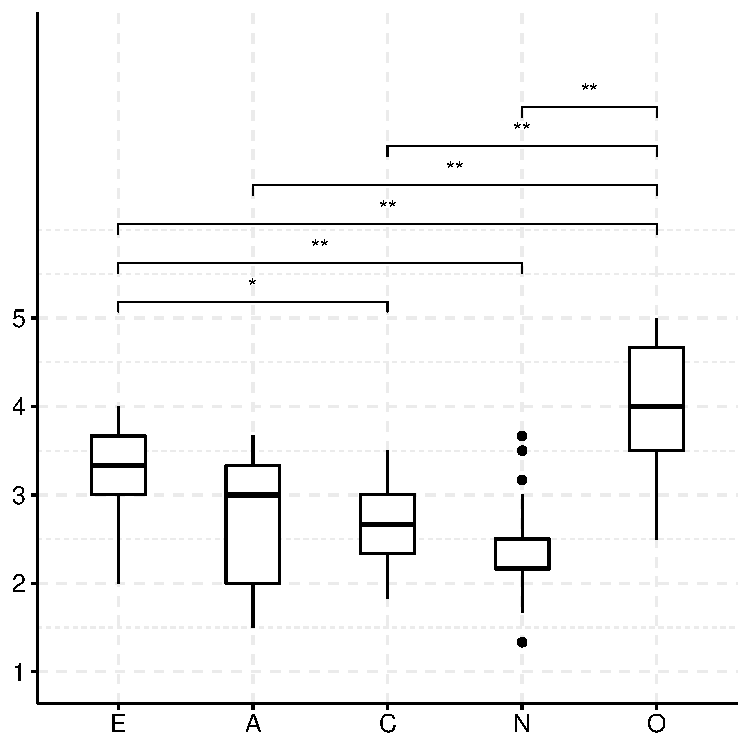
\includegraphics[width=1\linewidth]{M_T_Study_2_Yel.pdf}
        \caption{Yellow}
        \label{fig:sub1}
    \end{subfigure}\hfill%
    \begin{subfigure}{.45\textwidth}
        \centering
        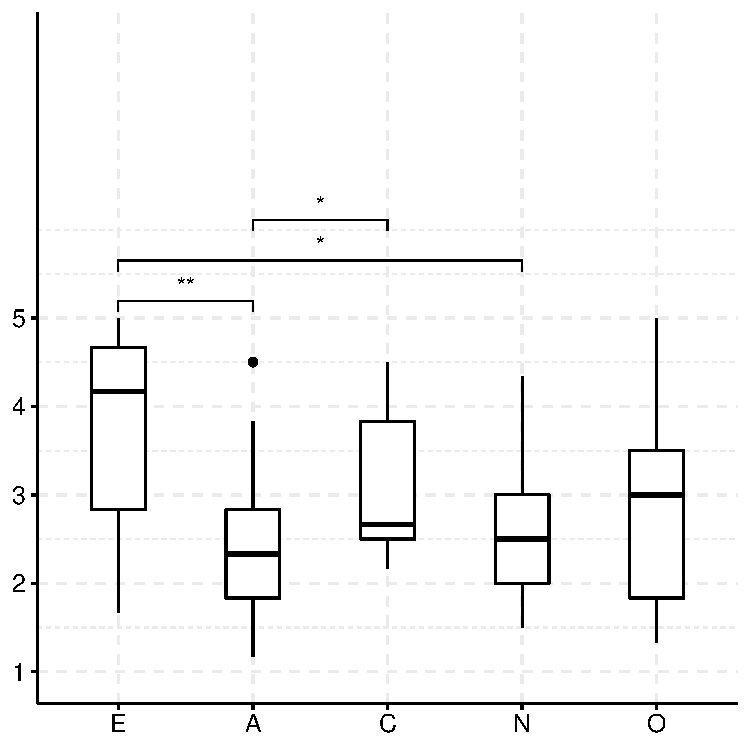
\includegraphics[width=1\linewidth]{M_T_Study_2_Oran.pdf}
        \caption{Orange}
        \label{fig:sub2}
    \end{subfigure}\hfill
    \begin{subfigure}{.45\textwidth}
        \centering
        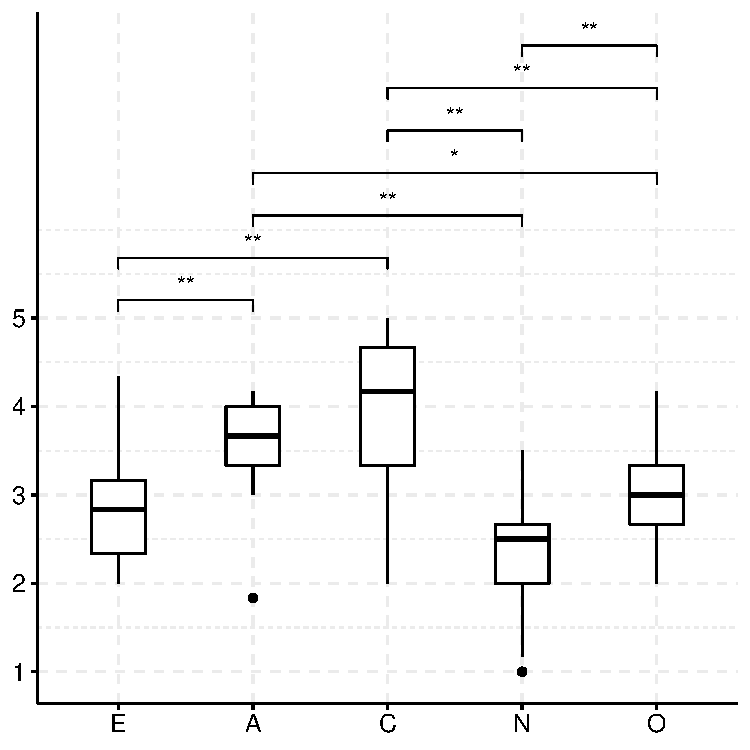
\includegraphics[width=1\linewidth]{M_T_Study_2_Tur.pdf}
        \caption{Turquoise}
        \label{fig:sub1}
    \end{subfigure}\hfill%
    \begin{subfigure}{.45\textwidth}
        \centering
        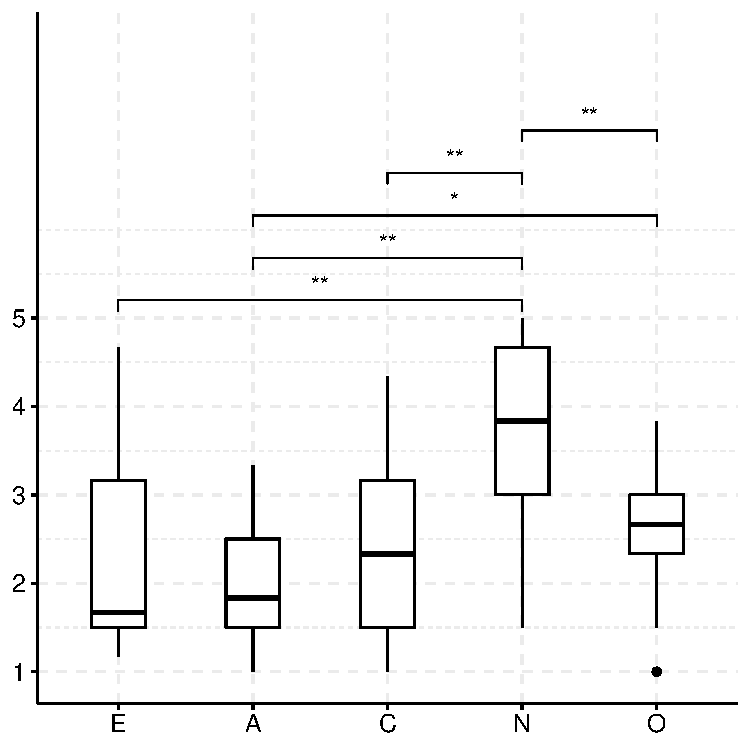
\includegraphics[width=1\linewidth]{M_T_Study_2_Blr.pdf}
        \caption{Blood-red}
        \label{fig:sub1}
    \end{subfigure}\hfill%
    \begin{subfigure}{.45\textwidth}
        \centering
        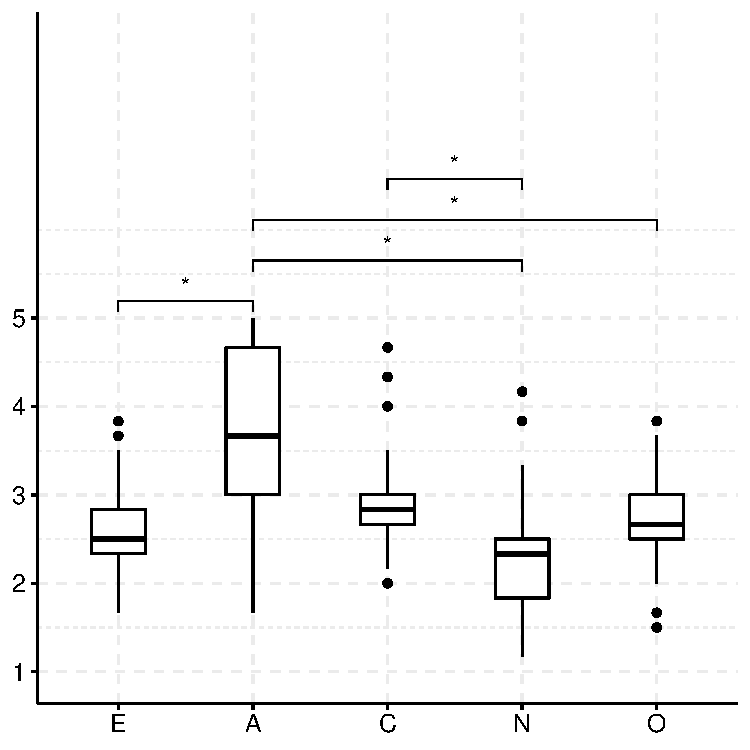
\includegraphics[width=1\linewidth]{M_T_Study_2_Pin.pdf}
        \caption{Pink}
        \label{fig:sub1}
    \end{subfigure}\hfill%
    \caption{A boxplot for the mascot-tablet interaction in study-2.
    Stars represent the significance of p\textsubscript{adj} after Bonferroni correction.}
    \label{fig:MT2}
\end{figure}

% TODO: Table median (values)
% TODO: Figure p-values
% TODO: p-value, df=?
% TODO: Med= or Med = , same for p<.1 or p < .1
